\documentclass[a4paper, 12pt, openright, oneside, german, french, english, brazil]{abntex2}
\usepackage[brazil]{babel}
\usepackage{graphicx}
\usepackage[utf8]{inputenc}
\usepackage{helvet}
\renewcommand{\familydefault}{\sfdefault}
\usepackage{wrapfig}
\usepackage{lscape}
\usepackage{rotating}
\usepackage{epstopdf}
\usepackage[alf,abnt-and-type=&]{abntex2cite}
\usepackage[a4paper, left=2cm, right=2cm, top=3cm, bottom=3cm]{geometry}
\usepackage{indentfirst}
\usepackage{longtable}
\usepackage{TikZ}
\pagestyle{plain}


\titulo{Projeto Pedagógico do Curso Superior de Tecnologia em Ciência de Dados}
\autor{Centro Universitário Metodista Izabela Hendrix}
\data{Abril, 2018}
\instituicao{Centro Universitário Metodista Izabela Hendrix}
\local{Belo Horizonte}

\begin{document}

\thispagestyle{empty}
	\begin{tikzpicture}[remember picture, overlay]
	\node[inner sep=0pt] at (current page.center) {%
		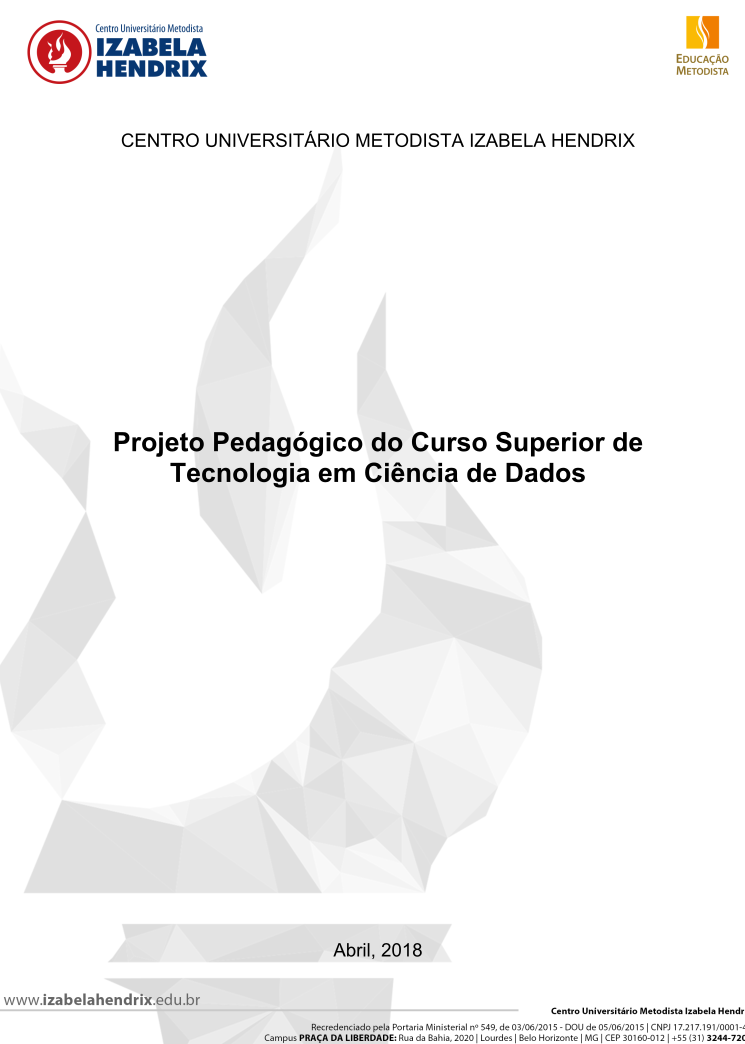
\includegraphics[width=\paperwidth,height=\paperheight]{capa_ppc_cd.png}%
	};
	\end{tikzpicture}
	\cleardoublepage{}
	
	
	\newpage
	

\pretextual
%\imprimircapa
%\listoffigures
%\listoftables
\newpage
\tableofcontents

\textual

\part{Contextualização}

\chapter{Dados de Identificação}

\section{Da Instituição Mantenedora}
\textbf{Nome:} Instituto Metodista Izabela Hendrix

\textbf{CNPJ:} 17.217.191/0001-40

\textbf{Endereço:} Rua da Bahia, nº. 2.020, Bairro Funcionários, Belo Horizonte – Minas Gerais.

\textbf{CEP:} 30160-012

\textbf{Telefone:} (31) 3244-7200

\textbf{E-mail:} reitoria@izabelahendrix.metodista.br

\textbf{Home page:} \url{http://www.izabelahendrix.edu.br}

\section{Da Instituição Mantida}
\textbf{Nome:} Centro Universitário Metodista Izabela Hendrix

\textbf{Endereço:} Campus Praça da Liberdade: Rua da Bahia, nº. 2.020, Bairro Funcionários, Belo Horizonte – Minas Gerais.

\textbf{CEP:} 30160-012

\textbf{Telefone:} (31) 3244-7200

\textbf{E-mail:} reitoria@izabelahendrix.metodista.br

\textbf{Home page:} \url{http://www.izabelahendrix.edu.br}

\section{Dos Dirigentes}

\textbf{Diretor Geral:} Robson Ramos de Aguiar

\textbf{Reitor:} Luciano Sathler Rosa Guimarães

\textbf{Diretoria Acadêmica:} Cecília Maria Carvalho Soares Oliveira

\textbf{Gestor Administrativo:} Marcos Antônio dos Reis


\chapter{Histórico}

\section{Histórico Institucional}

O Centro Universitário Metodista Izabela Hendrix faz parte de uma rede com mais de 700 universidades e colleges em todos os continentes, adota este estilo: valoriza sua memória, mas é original e projeta o futuro a cada instante.

O movimento metodista surgiu como renovação da Igreja Anglicana, na Inglaterra, na primeira metade dos anos 1700, durante a Revolução Industrial, dentro da Universidade de Oxford. Dali expandiu-se para outros continentes tendo ao lado de suas Igrejas uma escola e organizações de promoção humana\footnote{Ainda hoje existem, nas Igrejas Metodistas, as escolas dominicais voltadas para as crianças de até 12 anos.}. Revela, desde as suas origens, a concepção teológico-filosófica de unidade entre a prática da fé e a formação educativa para a vida social.

No Brasil, o processo de constituição de um sistema próprio de educação metodista tem origem no processo de inserção do protestantismo histórico no país; no contexto da abertura dos portos e substituição da mão-de-obra escrava pela mão-de-obra remunerada artesanal, manufatureira e laboral da imigração européia. O trabalho educacional era estratégia para o estabelecimento da Igreja no país, convicta de que a educação metodista ajudaria a libertação da ignorância, do analfabetismo e promoveria a modernização da sociedade, objetivando preparar as novas gerações para virem a ser futuras lideranças nacionais. As primeiras escolas metodistas se localizaram nos focos de presença da Igreja, nos Estados de São Paulo, Rio de Janeiro, Minas Gerais e Rio Grande do Sul.

O Izabela Hendrix foi criado em 1904, pela missionária norte-americana Marta Watts. No início, era um colégio destinado à educação de mulheres, o primeiro de Minas Gerais a reconhecer seus direitos e compreender a importância da atuação feminina na sociedade. Com mais de um século de existência, o Izabela Hendrix tem uma história que se mistura com a trajetória de Belo Horizonte. A capital mineira, com 110 anos apresenta em seu traçado e na sua gente a sofisticação e a ousadia de quem busca o novo sem deixar de ter raízes.

Hoje, o Instituto Metodista Izabela Hendrix é Colégio, Centro Universitário (Metodista de Minas), possui três campi e segue acreditando no poder transformador do ensino de qualidade. Com estrutura moderna e inteligente, professores(as) de alto nível e uma atuação arrojada no cenário educacional, orientada pelos princípios de uma sociedade mais justa e igualitária, a Metodista de Minas caminha para se tornar Universidade.

Mas estrutura e diretrizes não representam nada se não produzirem idéias e soluções inovadoras. Para isso, mais de 6.000 pessoas dão vida à Metodista de Minas. São estudantes, professores(as) e demais funcionários(as) que, junto à comunidade, usam laboratórios, bibliotecas, clínicas, auditórios, parque esportivo, capela, salas de aula e espaços de convívio como instrumentos que formam cidadãos e cidadãs e trazem melhorias para a sociedade.

Na tradição metodista, as escolas não são apenas lugar de estudar, sendo também espaços para viver. Além dos ambientes já citados, o Izabela Hendrix tem um teatro com 400 lugares, equipado com estrutura para a realização de eventos culturais e acadêmicos. Desde 2007, o Instituto conta com uma ampla biblioteca 24 horas, mais um projeto pioneiro que reafirma os ideais desta Casa, onde todo tempo é tempo de aprender e viver, onde a tradição é a base forte e a inovação é o caminho a percorrer.

\section{Histórico do Curso}

A \textit{Harvard Business Review} em um artigo de 2012 classificou a profissão de Cientista de Dados como ``\textit{the sexiest job of the 21st century}''. Essa explosão protagonizada por um profissional altamente capacitado e com formação multidisciplinar passou pela América do Norte, pela Europa e neste momento chega ao Brasil agitando o mercado das empresas consolidadas em todos os setores econômicos e \textit{startups}.

Apesar de toda a inquietação do mercado em relação à nova área, ainda é muito difícil conseguir profissionais com formação e habilidades adequadas ao trabalho. Isso se deve em parte ao fato de que a área requer uma construção de competências e habilidades altamente interdisciplinar envolvendo cálculo, estatística avançada, programação, bancos de dados e conhecimentos em negócios quanto à inexistência de um curso de graduação específico até a data da redação deste documento.

Assim, no primeiro semestre de 2018 foi inaugurado o Curso Superior de Tecnologia em Ciências de Dados do Centro Universitário Metodista Izabela Hendrix, o primeiro curso de graduação do Brasil nessa nova área. 

Alguém que deseja perseguir a carreira de cientista de dados deve buscar formação superior em Ciências Econômicas ou Matemática ou Estatística ou Ciências da Computação ou Ciências Sociais Aplicadas (com ênfase quantitativa) e depois buscar um MBA ou um mestrado específico na área. Desse modo, pretendemos deixar transparente a importância da criação do primeiro curso de graduação específico em Ciência de Dados do Brasil em que o aluno possa ter acesso aos diversos conteúdos a ele necessários e se desenvolver enquanto profissional com foco.


\chapter{Marco Referencial}

\section{Marco Referencial Institucional}

\subsection{A instituição}

O Centro Universitário Metodista Izabela Hendrix é uma instituição confessional, comunitária, privada. Sua natureza confessional reside em sua vinculação à Igreja Metodista, que entende a educação como ``o processo que visa a oferecer à pessoa e à comunidade uma compreensão da vida e da sociedade, comprometida com uma prática libertadora, recriando a vida e a sociedade, segundo o modelo de Jesus Cristo, questionando os sistemas de dominação e morte, à luz do Reino de Deus''\footnote{Diretrizes para a Educação na Igreja Metodista, Cânones da Igreja Metodista, 2002.}. A atuação educacional da Igreja Metodista não tem interesse pecuniário, nem desejo de proselitismo. Antes, é uma fidelidade para com sua vocação histórica e missionária.

Por sua vez, entendida a Igreja Metodista como uma comunidade missionária a serviço do povo, a natureza comunitária do Centro Universitário Metodista Izabela Hendrix origina-se de sua confessionalidade. Sua ação educativa, portanto, buscará sempre a melhoria das condições de vida no mundo e um posicionamento contra quaisquer tipos de preconceitos e ações de discriminação e exclusão.

Finalmente, sua natureza privada decorre do fato de ter sido instituída por uma entidade não governamental, dispondo, para sua manutenção e desenvolvimento, majoritariamente de recursos próprios.

\subsection{Missão}

A missão do Centro Universitário Metodista Izabela Hendrix é educar e formar cidadãos qualificados e críticos, com base em valores cristãos, para atuar na transformação da sociedade. Educar e formar revelam o desejo de transcender o processo educativo, que é muito centrado na pessoa, e buscar também o processo formativo, ou seja, a construção dos futuros cidadãos, conscientes de seus direitos e deveres e dotados de sólidos valores morais e éticos.

Por sua vez, o objetivo de formar cidadãos qualificados incorpora a dimensão da competência técnica, pois, parte importante da formação em nível superior é o “aprender a fazer”, isto é, a aquisição de competências específicas que vão definir o capacidade de pensar com autonomia e independência, exercendo juízo com acuidade.

A base dos valores cristãos está no cerne do Izabela Hendrix, como instituição confessional da Igreja Metodista, fundada por John Wesley - criador também da primeira escola metodista, a Kingswood School (1748 – Inglaterra) – que afirmava que ``ou teria uma escola cristã ou não teria nenhuma''. Ressalte-se que ser uma escola baseada em valores cristãos não significa dedicar-se ao proselitismo nem se mostrar intolerante para com pessoas de outras denominações e confissões religiosas. Pelo contrário, o princípio wesleyano era o ``pensar e deixar pensar''. Afirmar valores cristãos significa defender a justiça, a solidariedade, a cidadania, aspectos que o Izabela Hendrix considera imprescindíveis para que as pessoas sejam completas em sua formação.

Finalmente, a missão contextualiza o âmbito e o propósito da ação dos egressos da Instituição como para atuar na transformação da sociedade. A educação, no Izabela Hendrix, será sempre direcionada para gerar nos aprendentes o sentimento de inconformismo e o desejo por mudanças. O aluno que tem acesso à educação superior de qualidade precisa ter consciência de sua responsabilidade e compromisso para com os que não têm condições de ter o mesmo benefício.

\subsection{Práticas Educacionais}

A educação é uma jornada espiritual ou o processo de construção da verdade. Seu propósito essencial, a partir da aquisição do conhecimento, é religar o ser humano àquilo que de outro modo seria difícil ou inacessível, para inseri-lo, novamente, na grande trama da existência.

John Wesley, fundador do Metodismo, afirmava que “o propósito do conhecimento é permitir que os homens alcem seus pensamentos a objetos cada vez mais elevados e dignos de consideração, até ascenderem à fonte de todo o conhecimento, Deus”. Assim, em termos de suas práticas educacionais, o Centro

Universitário Metodista Izabela Hendrix busca os seguintes objetivos e características:

\begin{itemize}
\item Ser uma comunidade aprendente, elegendo o aluno como protagonista principal do processo educativo e não concebendo o professor como simples emissor de informa-ções, arcaísmo indesejado diante de um mundo saturado. Repudia-se o mero recurso à memorização como simulação da inteligência, entendendo que a inteligência é uma função que só se ativa na presença de uma situação-problema, exigindo flexibilidade e pensamento criativo.
\item Entender o desejo de conhecer como insaciável, ``um princípio fundamental no ser humano, inserido em sua natureza mais íntima.'' (John Wesley). 
\item Estimular o pensamento crítico como modo de participação do cidadão e a tolerância como meio de ouvir os outros sem perder a própria voz.
\item Promover a indissociabilidade entre ensino, pesquisa e extensão, ação que deve ter seu início na sala de aula, formando-se o aluno-pesquisador. Este deve ter na atividade de indagação o desafio para a descoberta de soluções novas.
\item Refletir, permanentemente, sobre a responsabilidade social do profissional formado em nível superior.
\item Conceber a interdisciplinaridade como forma de despertar o interesse e o compromisso dos alunos com o conhecimento, evitando-se a alienação causada pela frag-mentação dos conteúdos.
\item Incorporar em todas as suas práticas acadêmicas uma boa variedade de técnicas e recursos didáticos, sempre em busca do engajamento do aluno no processo de ensino-aprendizagem.
\item Incentivar reflexões sobre o papel das novas tecnologias na sociedade e no próprio processo de ensino-aprendizagem.
\item Conceber as práticas avaliativas como objeto fundamental para o desenvolvimento intelectual e pessoal do aprendente.
\end{itemize}

\subsection{Linhas Curriculares Institucionais - LCI's}

Uma visão mais consistente do endereçamento das políticas acadêmicas desencadeou o processo de definição das Linhas Curriculares Institucionais (LCIs). Para tal, o currículo foi entendido em sua visão macro, conforme o consagrado nessa área de conhecimento: isto é, tudo o que se produz no Centro Universitário Metodista Izabela Hendrix com a intencionalidade educativa. Assim, as LCIs nortearão o percurso de todos os cursos em suas atividades de ensino, pesquisa e extensão. Serão as grandes ênfases curriculares institucionais que refletirão, em síntese, qual é a intenção e missão da Educação Superior na Metodista de Minas.

As linhas, dentro das vocações da casa, devem expressar ao mesmo tempo os reflexos da história (o instituído) e o presente (instituído-instituinte), sinalizando o rumo que se quer imprimir às ações (instituinte de um ``novo'' instituído).

As LCIs não se confundem com a linhas de pesquisa ou áreas de conhecimento. Por serem mais amplas, as LCIs abarcam as linhas de pesquisa e as áreas de conhecimento e estende suas ações às linhas do ensino e da extensão. As Linhas Curriculares Institucionais são:

\begin{itemize}
\item Meio ambiente
\item Espaço Urbano
\item Responsabilidade social e formação cidadã
\item Gestão e Liderança
\item Empreendedorismo e inovação
\item Saúde coletiva
\end{itemize}

Dentro dos conteúdos da matriz curricular do curso de Ciência de Dados, serão trabalhadas as LCIs conforme descrito abaixo:

\begin{itemize}
\item Meio ambiente: entender a análise de dados ambientais dentro de uma visão sustentável;
\item Espaço urbano: compreender o espaço urbano dentro do contexto interno e externo à organização e suas implicações na gestão e tomada de decisão incorporando o conceito de \textit{cidades inteligentes};
\item Responsabilidade social e formação cidadã: formar e desenvolver um profissional com princípios de responsabilidade social, ética e cidadã;
\item Gestão e liderança: desenvolver competências sólidas para gerir e liderar pessoas e processos de maneira profissional com base em resultados;
\item Saúde coletiva: entender a importância da prevenção e saúde física e mental do trabalhador e sua produtividade na empresa;
\item Empreendedorismo e inovação: desenvolver o espírito empreendedor e o intraempreendedorismo, bem como capacitar o aluno para elaboração de um plano de negócio e tomar decisão.
\end{itemize}

As LCIs são eixos articuladores do conhecimento que permitem a convergência de práticas de ensino, pesquisa e extensão entre cursos, corpo docente e discente da institui-ção.

\section{Marco Referencial do Curso}

\subsection{O Curso Superior de Tecnologia em Ciência de Dados - Perfil do Profissional}

O Curso Superior de Tecnologia em Ciência de Dados é o primeiro curso de Graduação do Brasil; obedece as diretrizes contidas no parecer da Conselho Nacional de Educação (CNE)/Câmara de Educação Superior (CES) 436/2001; apresenta caráter formativo multidisciplinar, ultrapassando as áreas das ciências exatas; possui ferramentas que levarão o aluno a identificar, compilar, analisar e comunicar dados complexos para nas mais diversas áreas contribuindo para a melhoria da qualidade de vida e inovações no país.

Durante o curso, o aluno terá a certificação de sua capacitação durante os módulos (Art.5 CNE/CP 3/2002); obtenção de diploma de tecnólogo no término do curso; orientação prática em todas as disciplinas; e será capaz de induzir e participar do desenvolvimento em análise e processamento de dados do país, visando suprir a crescente demanda por profissionais capacitados em tecnologias alternativas para atuar na solução de problemas e criação de ferramentas básicas e aplicadas.

O desenvolvimento das capacidades profissionais do egresso será baseado na integra-ção da Educação, Ciência e Tecnologia, garantido a formação de cidadãos com competências profissionais inovadoras e éticas em prol do desenvolvimento do País.

As competências do egresso serão baseadas de acordo com a LDB (Lei 9394/96), o Decreto 5.591/2005 e o Art. 2 da CNE/CP3.

Durante o curso o aluno irá:

\begin{itemize}
\item Compreender os processos tecnológicos em suas causas e efeitos e desenvolver sua capacidade empreendedora;
\item Entender a importância da produção, inovação, gestão e incorporação científico-tecno-lógica para o mercado de trabalho, proporcionando a compreensão e avaliação dos impactos sociais, econômicos e ambientais resultantes;
\item Desenvolver competências profissionais tecnológicas, gerais e específicas, para a gestão de processos e a produção de bens e serviços;
\item Conscientizar sobre a importância do estudo contínuo (ex.: Pós-Graduação), aprimoramento das capacidades profissionais;
\item Entender a importância da interdisciplinaridade e atualização constante dos cursos e currículos;
\item Compreender as mais recentes ferramentas e tópicos de ciências de dados incluindo-se arquiteturas de \textit{Big Data}, captura e sistematização de dados, \textit{Data Mining}, Inteligência Artificial, os principais algoritmos de \textit{Machine Learning} e \textit{Deep Learning} e técnicas de visualização de dados;
\item Compreender a importância da ciência de dados na área das inovações tecnológicas, como no desenvolvimento de novos softwares e produtos;
\item Desenvolver competências com linguagens de programação como Python, R, entre outros;
\item Aprimorar uma carreira em ciências de dados, pesquisa, indústria, educação e ou desenvolvimento de software;
\end{itemize}

Sob o ponto de vista pedagógico, este projeto adotará as seguintes diretrizes:

\begin{itemize}
\item O currículo e o projeto pedagógico serão avaliados continuamente, visando subsidiar as correções necessárias;
\item A formação pretendida em Ciências de Dados tem caráter generalista e, para tanto, o currículo apresenta projetos integradores em todos os módulos, proporcionando visão interdisciplinar do Curso;
\item O currículo estimulará, em consonância com as particularidades das disciplinas, a realização de projetos de pesquisa, projetos de extensão e de atividades práticas que possibilitem ao aluno o acesso às diversas formas do conhecimento científico e sua aplicação na melhoria da qualidade de vida da comunidade. Serão também estimuladas as atividades que socializem o conhecimento produzido pelos corpos docente e discente;
\item Os conteúdos programáticos relativos às disciplinas e todas as atividades decorrentes destes estarão automática e permanentemente submetidas a uma análise crítica visando à identificação dos elementos essenciais (amplos) e acessórios (específicos); os primeiros terão o seu domínio garantido para cada área do conhecimento ou atua-ção;
\item Cada disciplina apresentará claramente, em seu plano de ensino, os seus objetivos gerais e específicos, os conteúdos, a metodologia de ensino e estratégias de avaliação;
\item Os estágios livres (não obrigatórios) nas diversas áreas de atuação do Cientista de Dados serão estimulados.
\end{itemize}

\subsection{Missão}

A missão proposta pelo Curso Tecnológico em Ciências de Dados do Centro Universitário Metodista Izabela Hendrix é a formação de profissionais cuja competência ultrapasse o âmbito das suas especialidades, sendo capazes de desenvolver projetos de pesquisa, produtos, novas metodologias de forma crítica e inovadora nas áreas de Inteligência Artificial, Big Data e Inteligência Organizacional. Suprindo a crescente demanda por profissionais capacitados em tecnologias alternativas para atuar na solução de problemas e criação de ferramentas básicas e aplicadas nas mais diversas áreas, contribuindo para a melhoria da qualidade de vida.

\subsection{Contexto atual da Ciência de Dados}

O Cientista de Dados é um profissional multidisciplinar que aplica técnicas da computa-ção, estatística e inteligência artificial no sentido de análise de dados para gerar informação e conhecimento nas mais diversas áreas.

O avanço da capacidade de armazenamento e processamento de dados das últimas duas décadas aumentou o número e a complexidade de dados gerados. O Cientista de Dados passou a exercer papel fundamental na criação, desenvolvimento e operação de banco de dados e outras ferramentas computacionais para coletar, organizar e interpretar dados.

Atualmente este profissional é capaz de trabalhar com aquisição de dados, processamento, armazenamento, distribuição, análise, interpretação e programação, com o objetivo de entender padrões e elaborar previsões com grande acurácia.

A atuação do Cientista de Dados no mercado de trabalho ou na carreira acadêmica tem acompanhado o crescimento da geração de dados e do processamento de informatização de empresas e centros voltados às áreas da indústria, agropecuária, inovação e pesquisas. A demanda por profissionais nesta área é grande, sendo considerada a grande profissão do futuro.

O profissional poderá trabalhar na área industrial, financeira, em centros de pesquisa, centros médicos, clínicas, órgãos públicos e empresas privadas.

\subsection{Perspectivas}

Este projeto pretende viabilizar condições (Art.7 CNE/CP 3/2002) para que os alunos do Curso Superior de Tecnologia em Ciência de Dados do Centro Universitário Metodista Izabela Hendrix possam efetivamente adquirir e colocar em prática a competência profissional pretendida de forma eficiente e eficaz requeridas para o desenvolvimento tecnológico.

Promover a formação de profissionais que visem os avanços tecnológicos, o aperfeiçoa-mento e as inovações para gerar ferramentas e produtos que contribuam para o desenvolvimento do país.


\chapter{Contextualização}

O curso Superior de Tecnologia em Ciência de Dados do Centro Universitário Metodista Izabela Hendrix pretende a formação integral de um profissional. Para tanto, precisa articular os saberes produzidos aos saberes necessários para a formação de profissionais. Estes saberes transcendem os relativos ao conteúdo das disciplinas. É fundamental que este sujeito seja despertado para a importância do seu papel na manutenção ou transformação da ordem social vigente.

Desta forma, é muito importante buscar a unidade dos saberes. Tratá-los de forma dual (científicos x senso comum, teóricos x práticos, racional x emocional), acaba por reforçar a dissociação, que fragiliza a formação.

É parte fundamental da contexto de aplicação deste projeto garantir o que preconiza a Lei de Diretrizes e Bases para a Educação Nacional quando define como fins da educação superior:

\begin{citacao}
  (\dots) estimular a criação cultural e o desenvolvimento do espírito científico e do pensamento reflexivo; formar diplomados nas diferentes áreas de conhecimento, aptos para a inserção em setores profissionais e para a participação no desenvolvimento da sociedade brasileira, e colaborar na sua formação contínua; incentivar o trabalho de pesquisa e investigação científica, visando o desenvolvimento da ciência e da tecnologia e da criação e difusão da cultura, e, desse modo, desenvolver o entendimento do homem e do meio em que vive; promover a divulgação de conhecimentos culturais, científicos e técnicos que constituem patrimônio da humanidade e comunicar o saber através do ensino, de publicações ou de outras formas de comunicação; suscitar o desejo permanente de aperfeiçoamento cultural e profissional e possibilitar a correspondente concretização, integrando os conhecimentos que vão sendo adquiridos numa estrutura intelectual sistematizadora do conhecimento de cada geração; estimular o conhecimento dos problemas do mundo presente, em particular os nacionais e regionais, prestar serviços especializados à comunidade e estabelecer com esta uma relação de reciprocidade; promover a extensão, aberta à participação da população, visando à difusão das conquistas e benefícios resultantes da criação cultural e da pesquisa científica e tecnológica geradas na instituição.\footnote{Ministério da Educação e Cultura, 1996.}
\end{citacao}

Acreditamos que a função social da formação profissional está voltada também para responder as demandas da sociedade, sejam elas advindas das indústrias ou do setor de serviços. É importante que seja superada a idéia de que as teorias sejam possíveis só no contexto acadêmico, mas, e principalmente, que a ciência esteja a serviço do desenvolvimento social.

Este projeto pedagógico pretende garantir que a graduação em Ciência de Dados seja uma etapa inicial, a base do processo de educação continuada. Para tanto, propomos que a formação integral do sujeito profissional requer sustentação por uma diversidade de espaços complementares de formação, sejam estes representados pelas atividades complementares, sejam constituídos pela convivência interdisciplinar.

O Curso Superior de Tecnologia em Ciência de Dados do Centro Universitário Metodista Izabela Hendrix foi idealizado tendo o paradigma da complexidade como norteador epistemológico. Isso reflete-se na lógica de organização da matriz curricular, que evita a linearidade, situação em que o conhecimento resultaria de uma sequência de disciplinas com conteúdos que dependiam necessariamente de uma disciplina anterior. Nossa proposta opta o quanto possível por uma lógica não linear, que pode ser compreendida sob dois aspectos.

No primeiro deles, todas as disciplinas do curso são divididas entre disciplinas de forma-ção básica e disciplinas de formação específica. Dentro da formação básica, desdobram-se duas dimensões. A primeira delas abarca um conjunto de disciplinas que trata da Relação ser humano-sociedade. A segunda formada pelo conjunto de disciplinas que irão promover a formação específica.

Tal dimensão é fundamental para o desenvolvimento do pensamento científico e por métodos investigativos que serão a base das relações com a busca pelo conhecimento e a informação.

Na formação específica encontram-se outras duas dimensões: a primeira delas, a dimensão Técnico-instrumental irá abarcar disciplinas que darão à esse aluno ferramentas didáticas para o trabalho com os conhecimentos específicos da área, levando em conta também os princípios de inclusão e acessibilidade aos seus alunos. Finalmente, a dimensão prático-pedagógica contempla a disciplinas que contribuem para a mediação do conhecimento e a atuação profissional, tal como os estágios e práticas como componente curricular, responsáveis por aproximar os alunos da realidade de atuação na sociedade.

Uma formação que não pretende ser linear requer que mesmo os espaços tradicionais do processo de formação sejam repensados. A sala de aula deve ser pensada como a menor unidade deste processo; ela deve ser reconhecida como o endereço, como o local de referência para um sujeito em formação. Este espaço deve ser ocupado por um conjunto de iguais; um local de onde todos irão partir; um local onde se reencontrarão em diferentes etapas da caminhada; um local onde a diversidade será reconhecida como potencialidade e as especificidades como complementares. A pesquisa, por sua vez, deverá orientar, instigar, despertar o espírito explorador da natureza humana; deve dar a direção e os instrumentos para a busca de conhecimentos e a produção do novo. Ela deve ser adotada como uma dimensão do processo de formação, um elemento imprescindível à formação que se pretende.

A articulação dos conhecimentos pode ser explicitada na prática de pesquisa. Para além de aprenderem a metodologia de pesquisa é fundamental que vivenciem o processo da pesquisa desde a exploração do tema até o produto final. Esta ideia de que a pesquisa é uma prática para poucos ou que existem os que pensam, pesquisam e produzem conhecimentos e os que executam, deve ser superada, pois pode ser mais um elemento de reforço da dissociação do conhecimento e da fragilidade da formação profissional.

Os laboratórios e espaços específicos do curso precisam ser locais de convivência e de troca interdisciplinar, onde as diversas áreas do saber possam cooperar, onde aprendam a conviver de forma harmônica e solidária como cidadãos e onde aprendam a compartilhar as descobertas e comungar os sucessos e insucessos, onde reconheçam que as respostas e o conhecimento ora produzido são provisórios, onde a verdade não existe como absoluta, onde a teoria se materializa, onde enfim possamos nos reconhecer como iguais.

\chapter{Perspectivas}

Com a implantação do Curso Superior de Tecnologia em Ciência de Dados o Centro Universitário Metodista Izabela Hendrix alia a tradição metodista com sua missão social, se comprometendo com a formação de profissionais que atenderão às necessidades da sociedade de forma crítica e criativa.

A implantação deste curso amplia a oferta de cursos, mostra um reposicionamento da imagem da instituição, e incentiva o desenvolvimento de mecanismos de promoção e difusão cultural e artística articulando as comunidades Izabelina e a local.

A localização do Campus Praça da Liberdade, no qual estão situados também os cursos de Bacharelado em Engenharia da Computação, Engenharia de Produção, Engenharia Civil, Engenharia Ambiental e Sanitária, Arquitetura e os cursos Tecnológicos de Bioinformática e Design de interiores, favorece o acesso aos trabalhadores e estudantes de toda a região metropolitana, onde cumpre importante papel social.


\part{Do Curso}

\chapter{Dados sobre o curso}

\section{Regulamentação Legal do Profissional}

O profissional Tecnólogo em Ciência de Dados formado pelo Centro Universitário Metodista Izabela Hendrix receberá o título Tecnólogo em Processamento de Dados (2124-05 da CBO). De acordo com Art. 5 da CNP/CE 3/2002: ``O concluinte de módulos correspondentes a qualificações profissionais fará jus ao respectivo Certificado de Qualificação Profissional de Nível Tecnológico''.

Compete ao Profissional Tecnólogo em Ciência de Dados desenvolver todos os itens propostos no Art. 2 da CNE/CP3, além de projetos de pesquisa, produtos, novas metodologias de forma crítica e inovadora nas áreas de \textit{Big Data}, \textit{Machine Learning} e \textit{Deep Learning}, suprindo a crescente demanda por profissionais capacitados em tecnologias alternativas para atuar na solução de problemas e criação de ferramentas básicas e aplicadas nas mais diversas áreas contribuindo para a melhoria da qualidade de vida.

\section{Integralização}

De acordo com a CNE/CES 02/2007 que versa sobre o tema ``Duração dos Cursos de Educação Superior'': a figura da modalidade de tecnólogo como graduação de natureza especial, contempla cursos cuja duração, fixada em horas, varia entre 1.600 horas e 2.400 horas.

O CST em Ciências de Dados do Centro Universitário Metodista Izabela Hendrix, apresenta 2.000 horas divididas em cinco módulos, ou seja, dois anos e meio.

\section{Número de Vagas}
Serão ofertadas semestralmente 60 vagas, sendo 30 vagas no turno matutino e 30 vagas no turno noturno.

\section{Turno de Funcionamento}
O curso será oferecido de segunda-feira a sexta-feira, com turmas em funcionamento no período matutino e turmas no período noturno. As turmas de ambos os turnos poderão ter aulas aos sábados pela manhã.

\chapter{Objetivos do Curso}

O Curso Superior de Tecnologia em Ciência de Dados do Centro Universitário Izabela Hendrix tem como objetivo formar o profissional ético e competente, capaz e agir em sua sociedade, induzir e participar do desenvolvimento do país, visando suprir a crescente demanda por profissionais capacitados em tecnologias alternativas para atuar na solução de problemas e criação de ferramentas básicas e aplicadas na mais diversas área, contribuindo para a melhoria da qualidade de vida.

\chapter{Perfil do Profissional Formado pelo Centro Universitário Metodista Izabela Hendrix}

Educar e formar cidadãos qualificados e críticos, com base em valores cristãos, para atuar na transformação da sociedade é parte da missão do Centro Universitário. Entretanto, a formação crítica não se completa sem uma reação propositiva. A reação à crítica deve ser traduzida numa alternativa, numa solução, numa proposta criativa de superação de uma situação-problema.

O cidadão criativo atua em prol de estilos de vida sustentáveis. Busca soluções alternativas para problemas comuns ao dia-a-dia, voltados para um padrão de bem-estar social, baseado em produtos e serviços sustentáveis, que viabilizem soluções eficientes e acessíveis para o cotidiano das pessoas. São práticas de inovação social sustentável que, aplicadas ao cotidiano, propiciam novos modos de vida responsáveis.

\section{Competências e Habilidades Comuns}

Espera-se que todo aluno formado pelo Centro Universitário Metodista Izabela Hendrix tenha competência para:

\begin{itemize}
\item Pensar criticamente, resolver problemas e tomar decisões, com disposição e responsabilidade para assumir riscos e propor soluções criativas;
\item Filtrar e separar, na grande massa de informações disponíveis, o útil do inútil, discernindo entre o importante e o supérfluo, com autonomia para dar continuidade, ao longo de toda vida, ao seu processo de aprendizado;
\item Viver e trabalhar com efetividade e confiança em uma sociedade de informação, dentro de uma comunidade global, respeitando e valorizando as diferentes culturas;
\item Adquirir uma sólida cultura geral e espírito enlevado, transcendendo a mera formação para o exercício de uma profissão;
\item Trabalhar em grupo respeitando e valorizando os diferentes pontos de vista, benefician-do-se deles e colaborando para a integração das diferenças em prol de um bem-estar coletivo sempre em construção;
\item Exercitar a solidariedade e a alteridade, seja individualmente, seja coletivamente, assumindo sua responsabilidade social, como egresso do ensino superior;
\item Colaborar na construção do saber e para repassar o conhecimento às comunidades científicas e leigas, contribuindo com os cidadãos nos seus direitos de acesso e uso da informação;
\item Denunciar com prontidão todo e qualquer tipo de discriminação ou dominação que marginalize a pessoa humana e ameace a existência de seres vivos;
\item Apoiar os movimentos que visem à libertação dos oprimidos e o acolhimento dos excluídos, bem como o acesso seguro e saudável aos ambientes onde manifestam sua cultura;
\item Comunicar-se com bom uso do português, com vocabulário rico e baseado em uma compreensão profunda da linguagem e da condição humana.
\end{itemize}

\section{Competências e Habilidades Específicas do Curso}

O Tecnólogo em Ciência de Dados formado pelo Centro Universitário Metodista Izabela Hendrix é um profissional com sólida formação científica, capaz de usar o conhecimento específico desta área para atuar nos mais diversos espaços. Sendo assim, para além das competências gerais dos egressos do Centro Universitário Metodista Izabela Hendrix, aqueles formados no Tecnólogo em Ciência de Dados deverão ainda estarem aptos para:

\begin{itemize}
\item Identificar e utilizar os diversos conteúdos da cultura do movimento humano, estimulando a criatividade, a reflexão e a compreensão histórica destes conteúdos;
\item Ter uma concepção consciente e clara do significado e dos objetivos de suprir a crescente demanda por profissionais capacitados em tecnologias alternativas para atuar na solução de problemas e criação de ferramentas básicas e aplicadas nas mais diversas áreas, contribuindo para a melhoria da qualidade de vida;
\item Ter uma concepção consciente e clara de sua atuação em prol do bem-estar e da qualidade de vida das pessoas.
\item Exercer papel fundamental na criação, desenvolvimento e operação de banco de dados e outras ferramentas computacionais para coletar, organizar e interpretar dados, visando sempre o desenvolvimento tecnológico da instituição envolvida e do país;
\item Trabalhar com aquisição de dados, processamento, armazenamento, distribuição, aná-lise, interpretação e programação com o objetivo de entender padrões nos dados dentro dos princípios éticos e sociais.
\end{itemize}

\chapter{Práticas de Ensino}

O ensino é uma das dimensões que possibilita a democratização e o acesso ao conhecimento elaborado, transformando-o em ações práticas de intervenção no meio social e no mundo do trabalho. Nesse contexto, o conhecimento aparece como mediação do poder e como ferramenta da criação de símbolos através de um processo de intencionalização técnica e política, deixando de ser mecânica, projetando o trabalho como sentido.

Daí se esperar da educação que ela constitua, em sua efetividade prática, um decidido investimento na consolidação das forças construtivas dessas mediações. Impõe-se garantir que a educação seja mediação da percepção das relações situacionais, que ela lhes possibilite a apreensão das intrincadas redes políticas da realidade social, pois só a partir daí poderão se dar conta também do significado de suas atividades técnicas e culturais.

Cabe ainda à educação desvendar os mascaramentos ideológicos de sua atividade, evitando assim que se instaure como mera força de reprodução social e se torne capaz de vir a ser força de transformação da sociedade, de tantas maneiras quantas as permitidas pela criatividade de mentalidades preparadas e abertas para a sensibilidade do social, capazes de propor e executar alternativas que projetem as comunidades a outros patamares de qualidade de vida. Visão esta não ingênua de que a educação pode, sozinha, dar conta de fazer a transformação da sociedade, mas a de que o que lhe compete fazer não deve deixar de ser feito. Assim o Izabela Hendrix oferece uma educação responsável por proporcionar formação de cidadãos(ãs) comprometidos(as) com as práticas da responsabilidade social, e com atitudes solidárias, como respostas de quem é educado.

Propõe-se nortear as práticas de ensino do Centro Universitário pelos seguintes conceitos:

\vspace{5mm}

\textbf{a. Práticas de ensino inclusivas}

Conscientes de que o acesso à educação superior no Brasil ainda é privilégio de uma pequena parcela da população brasileira com idade entre 18 e 24 anos o Izabela Hendrix lida com um dado de realidade que se torna ponto chave na releitura dos seus princípios vocacionais. Sendo uma instituição confessional e filantrópica, parte desta vocação, em princípio, está estruturada, como o demonstrado neste PDI, pela própria natureza da instituição, ou seja, destinar a filantropia à distribuição de bolsas de estudo.

Estas bolsas são distribuídas em várias modalidades e finalidades, tais como o PROUNI, capacitação de funcionários(as), cotas de bolsas destinadas à minorias vinculadas a movimentos sociais e a programas de intercâmbio internacionais (PEC-G, PAI e outros). Deste modo entende-se que a inclusão passa, na educação, pelo acesso à formação e à capacita-ção de jovens e adultos que por muitas razões não tiveram acesso à educação superior de qualidade.

Mas o entendimento de inclusão e as políticas e práticas institucionais não se limitam à distribuição de bolsas. A inclusão passa também por abordagens pedagógicas postas em prática nas diversas formas de aula, nos princípios que norteiam a organização e implementação curricular, expressos nos Projetos Pedagógicos dos Cursos, nas mediações exercidas por todos(as) os(as) responsáveis aos atendimentos dos(as) alunos(as), nas muitas atividades, projetos e programas que interligam e indissociam o ensino, a pesquisa e a extensão, nas dinâmicas que entrelaçam o acadêmico ao administrativo, numa vivência colegiada e democrática que exercita vida comunitária-cidadã, nas parcerias estabelecidas para a concretização de nossos ideais acadêmicos, na cordialidade no trato e na vivência cotidiana da experiência de se trabalhar num Centro Universitário, no respeito às diferenças e na não-discriminalização de pessoas, na integração entre os níveis de ensino: educação básica e superior, entre outras.

Exemplos dessas concepções e de suas práticas podem ser percebidas na:

\begin{itemize}
\item Organização de um currículo concebido como de qualidade, entendida como o não abrir mão do que é essencial e deve ser sólido na formação do profissional das áreas, generalista, porque possibilita uma formação abrangente da problemática que envolve os contextos micros e macros sociais onde se inserem a profissão, mas adensada e adequada à rapidez da atualidade e consoante com as melhores tendências internacionais contemporâneas de duração de cursos, numa sociedade prenhe de recursos e técnicas que interagem, complementam e dão dinâmica própria às aprendizagens significativas, em todos os campos do conhecimento. Entendendo que a profissionalização na graduação e a especialização devem ser focadas como um continuum, dentro da visão de educação inicial e continuada, ensejando e motivando a pós-graduação lato e stricto sensu, concernente à visão de que educação é para a vida e por toda a vida, os Projetos Pedagógicos dos Cursos demonstram e trazem em seu interior essas concepções. Hoje a resposta às exigências de uma formação mais rápida não é contraditória à constatação de que os(as) jovens adentram a universidade em idades cada vez mais tenras e de que necessitam maior tempo para amadurecer sua formação acadêmica. Ao contrário, garante que variáveis e esforços pessoais possam ser atendidos e aparecem como estratégias sensíveis para entender que o(a) aluno(a) trabalhador(a), que compõe a maioria do Centro Universitário (que é particular e confessional), estuda à noite por falta de opção. Muitos(as) ainda têm responsabilidades familiares, devem ver suas necessidades respondidas como um direito que possuem a uma formação de igual qualidade que a dos(as) estudantes do diurno. Que por essa e outras razões tenha uma boa formação que lhe possibilite adentrar rapidamente no mercado de trabalho e seja produtivo, podendo concorrer em condições de igualdade com os(as) estudantes que se formam no diurno. Entende-se, desta forma, que os cursos noturnos têm a mesma qualidade que os oferecidos durante o dia, em que pese que os(as) alunos(as)-trabalhadores(as) do noturno tenham que despender mais esforços pessoais em sua formação e qualificação profissional. Assim é compreensível que um semestre a mais na duração de um curso para este(a) aluno(a) pode significar uma evasão por exaustão pessoal ou por motivos de comprometimento alongado de sua capacidade de comprometimento de seus recursos financeiros. Não agir assim significa presenciar e ser conivente passivamente com outras formas de exclusão mais sutis, imperceptíveis e perversas por tratar-se de excluir quem chegou ao Ensino Superior, ou seja, teve o acesso, mas não as condições para a permanência e conclusão de sua educação superior.

\item Viabilização de horários flexíveis e adequados ao ritmo e empenho pessoal de cada aluno(a). Cada aluno(a) tem o seu tempo de dedicação pessoal, e seu ritmo próprio de aprendizagem que écondicionado por diversos fatores pessoais, de ordem familiar e/ou profissional. Ao incluir disciplinas em EAD e/ou semi-presenciais, bem como atividades de trabalho independente em locais e tempos diferenciados, o Izabela Hendrix tem em vista que está lidando com instrumentos pedagógicos capazes de flexibilizar o curso e garantir que os momentos de formação não sejam medidos apenas pela organização rígida de horários semanais de aula, nem pelo espaço propiciado apenas pela escola para que dê conta de suas atividades e estudos, bem como de suas aplicações práticas.
\end{itemize}

\vspace{5mm}

\textbf{b. Práticas pedagógicas expandidas e consequente formação de outros espaços de aprendizado}

No Izabela Hendrix está claro que o ensino não está dissociado da pesquisa e da extensão. Desta forma, não se pode ter a pesquisa e a extensão dos cursos como práticas diversas do cotidiano de aprendizagem. Neste sentido é preciso pensar em renovar, expandir e repensar constantemente as práticas pedagógicas e constantemente recriar os espaços de aprendizado. O incentivo às práticas pedagógicas expandidas e a formação de outros espaços de aprendizado depende da concepção dos sujeitos da pesquisa, dos sujeitos da extensão, dos sujeitos do ensino, estes sujeitos que fazem parte da vida acadêmica, sujeitos do saber, alunos(as) e professores(as) são os(as) que não dissociam as práticas ensino-pesquisa-extensão.

Os sujeitos do saber não têm apego às tradições e ao conforto. Incomodam-se com a permanência, negam práticas conteudistas e não se limitam às organizações funcionais da universidade. Os sujeitos do saber reconhecem as linhas curriculares institucionais e as políticas institucionais, mas também têm a capacidade de perceber que o currículo e a ementa de uma determinada disciplina, por exemplo, não devem ser apenas uma encomenda pontual e fragmentada de um momento do curso a um(a) professor(a) que entra e depois poderá ser substituído(a) por outro(a).

A instituição, por mais que seja estruturada como tal, não deseja ser uma linha de reprodução funcionalista, ou fordista. As Linhas Curriculares, os Projetos e as Políticas Institucionais são um foco comum, uma diretriz de ação que permite uma identidade/autônoma aos sujeitos do saber PARALELO às organizações funcionais inerentes e necessárias à uma instituição. A organização funcional se constitui de rumos, focos e meios para se potencializar numa prática coletiva. É um acordo coletivo PARA A PRODUÇÃO COMUM.

Não se pode confundir a prática dos sujeitos do saber com a organização funcional. O sujeito do saber independe da organização funcional. A prática de ensino dos sujeitos do saber ocorre em qualquer instância, em qualquer espaço, tempo, lugar, com ou sem recursos. O fim da instituição é somar o potencial individual de cada um destes sujeitos dando corpo a uma universidade, no seu melhor sentido de universalizar idéias e ideais, com universos pessoais diferentes e diferenciados, que se dirige a um universo do alunado dispare e por isso mesmo rico e pleno de possibilidades de realização e de criação de coisas novas. Traz em si o desafio de se repensar a educação, a sociedade, as próprias possibilidades e suas concretudes. No Izabela Hendrix a formação não se limita a um grupo de disciplinas, da exposição e consumo de conhecimentos, do aprender de uma técnica e/ou um saber fazer específico. São desenvolvidos espaços de aprendizado capazes de interferir na formação, o que permite ao conhecimento se transformar num procedimento cotidiano, numa prática cada vez mais vinculada à rotina do sujeito do saber. Desta forma a extensão, a pesquisa e a pós-graduação assumem responsabilidades com cada um(a) dos estudantes em programas de graduação.

\vspace{5mm}

\textbf{c. Formação de cidadãos críticos, criativos e socialmente responsáveis}

Educar e formar cidadãos(ãs) qualificados(as) e críticos(as), com base em valores cris-tãos, para atuar na transformação da sociedade é parte da missão do Centro Universitário. Entretanto, a formação crítica não se completa sem uma reação propositiva. A reação à crítica deve ser traduzida numa alternativa, numa solução, numa proposta criativa de superação de uma situação-problema. O(A) cidadão(ã) criativo(a) atua em prol de estilos de vida sustentáveis. São cidadãos(ãs) que buscam soluções alternativas para problemas comuns ao dia-a-dia, voltados para um padrão de bem-estar social, baseado em produtos e serviços sustentáveis, que viabilizem soluções eficientes e acessíveis para o cotidiano das pessoas. São práticas de inovação social sustentável aplicados ao cotidiano e propiciando novos modos de vida responsáveis.

\vspace{5mm}

\textbf{d. Uma comunidade de aprendizado contínuo}

Uma comunidade de aprendizado continuo assume o compromisso de se atualizar e renovar o conhecimento permanentemente. Estas práticas devem promover o contato com o egresso que não apenas retorna para buscar novos conhecimentos, mas também para compartilhar experiências e renovar as perspectivas de formação profissional e humana. Desta forma os programas de extensão, a pós-graduação lato sensu e o stricto sensu são práticas estratégicas de aprendizado contínuo e de trocas entre alunos(as), egressos e sociedade.

A educação continuada na perspectiva proposta aqui contribui com a especialização e inserção do egresso em práticas profissionais específicas e contextualizadas por demandas, às vezes temporárias do mercado. Desta forma, a instituição consegue uma inserção flexível de mercado impulsionando dinâmicas que são diferenciadas da graduação.

Dinâmicas das práticas pedagógicas (ensino, pesquisa, extensão e internacionalização). Em um processo de construção inventiva/propositiva do conhecimento, certas separações a priori, podem formalizar/enquadrar, simplificando o processo de desenvolvimento de uma formação. Se forem separadas a prática do pensamento, corre-se o risco de apostar em modelos que talvez não mais respondam a uma realidade veloz e em constante transformação como a atual. Daí uma prática de ensino construída diariamente. Uma prática contínua de formação, através da busca de uma construção cúmplice de um saber/fazer repensado a cada ato construtor: a necessidade de sempre ser mais inventivo durante o processo de curso da formação profissional.

Constantemente buscar propor instâncias de aberturas e flexibilizações para que estas investigações necessárias possam constantemente acontecer são comportamentos incentivados no corpo docente. O criar e recriar a temática da “aula”, o problematizar questões do cotidiano, notícias dos jornais, revistas e telejornais, a busca de outros espaços e tempos de aprendizagens significativas são algumas das possibilidades que contribuem para que esse processo de construção e produção de saberes se realize de forma mais prazerosa, mas não menos dedicada a exigir esforços dos sujeitos-aprendentes, como cada ser humano.

Para uma proposta pedagógica que se faz com ênfase na realidade regional e brasileira afetada pelas subjetividades atuais, propõe-se no Izabela Hendrix como práticas de pesquisa a abordagem de situações empíricas do cotidiano local como campo para onde convergem a crítica e as proposições. Se o objetivo da teoria é alterar a prática ou questioná-la, a abordagem de situações-problema presentes na sociedade busca construir uma crítica propositiva, fundamentada pelas experiências do mundo real onde esses(as) profissionais irão atuar. Tais estudos desenvolvem-se por entre os fluxos da teoria e da prática; a história atualizada por um devir de uma dada experiência, as observações empíricas problematizadas pelo conhecimento teórico devidamente atualizado. Nessa direção, faz-se necessário desenvolver convênios, parcerias com o poder público, com setores da economia privada, universidades (privilegiando-se a intercomplementaridade) ou demais instituições de ensino, cooperativas, ONGs, grupos organizados da sociedade civil elencando-se possibilidades diversas de associações de acordo com a especificidade da situação e da abordagem que se pretende.

O objetivo maior é de se criar um campo de reflexão, prospecção e debate animado pela heterogeneidade de deveres do cotidiano da nossa sociedade para quem os(as) estudantes apresentam planos de ações, proposições, invenções respondendo ou problematizando as demandas endereçadas.

As práticas de extensão estão intimamente relacionadas às práticas de ensino e de pesquisa, conformam uma rede e estão fundamentalmente implicadas com a sociedade, com a economia e com a cultura.

A extensão é pensada intrínseca às práticas de ensino, isto é, há uma organicidade estrutural entre as atividades realizadas nas disciplinas teóricas, práticas, tecnológicas e a extensão. A proposta é uma fusão entre essas experiências dentro das possibilidades e flexibilidades de cada campo. A abordagem de situações-problemas reais como temas a serem desenvolvidos nas disciplinas nos evocam e possibilitam que esses sejam tratados no campo da extensão, posto que nascem de necessidades da realidade. A ideia é que “sala de aula” e extensão se sobreponham às atividades de pesquisa e constituam um só corpo. Esse conjunto de agenciamentos que constituem as situações reais são problematizados pelos(as) professores(as) e estudantes que transitam por entre a escola, e os diversos setores da sociedade. Espera-se, assim, contribuir para um processo de construção do conhecimento não encerrado nos limites da escola, mas fazendo dessa uma potencializadora de dispositivos que estendam as possibilidades de ação dos(as) estudantes na sociedade. Essa proposta requer uma atenção especial às suscetibilidades do meio, bem como uma habilidade na captação de parceiros das mais diferentes esferas.

\chapter{Práticas de Pesquisa}

A pesquisa no Izabela Hendrix é entendida tanto em seu sentido stricto como lato, ou seja, no dizer de DEMO (1995): como um princípio científico e educativo. Assim é entendida como busca, indagação de respostas aos problemas que a realidade impõe ao cotidiano acadêmico, e como dever de ofício, dever dos(as) que se dedicam a fazer da docência, mais do que o exercício de uma profissão regulamentada, por estar comprometido com o devir de realidades, que se sente na obrigação de contribuir para modificá-las, alterá-las, pelo fazer diário.

Ser docente-pesquisador(a) é buscar respostas para as demandas que o alunado e as comunidades do entorno institucional apresentam; é sentir-se desafiado a criar alternativas que apontem outras construções possíveis ao que a realidade apresenta; é sentir-se instigado pelo cotidiano e ser um(a) instigador(a), incitando o alunado a acompanhá-lo(a) nessa travessia criadora e, por vezes, transgressora. É não aceitar o óbvio como um dado pronto e acabado, mas estar atento às oportunidades de fazer diferença em seu local de trabalho e em sua comunidade. É estar compromissado com uma educação dialógica e emancipadora, rica em oportunidades para se fazer diferente, tão necessário às nossas comunidades e a este país continente, pleno de desafios sociais.

Por isso, integrada ao ensino e à extensão, a pesquisa é aqui pensada como forma de proporcionar e orientar o desenvolvimento institucional, propiciando interfaces com as questões sociais, norte de intervenção e responsabilidade social do Izabela Hendrix. Implantada em todos os cursos, como parte do processo de se aprender permanentemente, e associada à extensão, a pesquisa é considerada um dos pilares da educação de qualidade e o principal motor incentivador da qualificação docente e discente.

A pesquisa como princípio formativo e epistemológico, eixo da organização e desenvolvimento curricular em ambiente universitário poderá garantir condições para uma efetiva contribuição cidadã ao corpo discente, como sujeito aprendente, no contexto de seu ingresso no espaço social de produção e reprodução de conhecimento em que se estabelecer. A política atual de pesquisa e iniciação científica orienta-se pela busca de sua institucionalização, como uma das formas para se consolidar este Centro Universitário, em sua trajetória de transformar-se em Universidade.

As atividades de pesquisa do Centro Universitário Metodista Izabela Hendrix estão vinculadas à Reitoria e são coordenadas pela Assessoria de Pesquisa e Intenarcionalização, por meio das ações dos(as) Coordenadores(as) de Cursos, dentro da estrutura e compreensão de que é no curso que deve nascer e articular-se toda a vida acadêmica.

A Assessoria de Pesquisa e Internacionalização em articulação com as coordenações de cursos, interage com os corpos docente e discente, com outras instituições congêneres e organismos voltados para a pesquisa, construindo e atualizando, implementando, acompanhando e avaliando as políticas da área. A instituição conta ainda com um Comitê de Ética, com suas funções próprias delineadas e aprovadas pelo CONSUN.

Em seus esforços para implementar e estimular a realização de atividades de pesquisa o Centro Universitário adota as seguintes práticas institucionais:

\begin{itemize}
\item apoio institucional à realização das atividades de pesquisa, englobando aporte financeiro, humano, físico e tecnológico;
\item busca de novas fontes de recursos financeiros para auxílio à iniciação científica e à pesquisa, como meio de potencializá-las;
\item auxílio à qualificação dos docentes perseguindo a meta de se ter um corpo de profissionais formado por mestres e doutores;
\item busca da consolidação do PIEPE – Programa de Incentivo ao Ensino, à Pesquisa e à Extensão;
\item orientações para a escolha e seleção da temática dos trabalhos de pesquisa e extensão em sintonia com as necessidades e demandas da sociedade do entorno dos campi, expressas nas Linhas Curriculares Institucionais;
\item promoção de intercâmbio com instituições científicas, nacionais e estrangeiras, visando desenvolver projetos conjuntos e troca de experiências com outros(as) pesquisadores(as);
\item ampliação e consolidação da busca de parcerias com vistas a desenvolver atividades de pesquisa;
\item incentivos à divulgação e publicação dos resultados científicos dos seus estudos e pesquisas;
\item estabelecimento de projetos que atendam as Linhas Curriculares Institucionais (LCIs) e que ensejem pesquisas estimuladoras da transdisciplinaridade e da integração entre cursos e áreas de saber;
\item fomento de pesquisas voltadas ao atendimento da demanda social;
\item articulação da elaboração dos Trabalhos de Conclusão de Curso (TCC), de graduação e pós-graduação lato sensu às LCI’s, coletivamente estabelecidas.
\end{itemize}

A institucionalização da pesquisa e da iniciação científica contribui para o desenvolvimento de formas de pensamento que asseguram aos(às) acadêmicos(as) maior clareza em seus modos de pensar e ver o mundo, com poder crítico, construtivo e independente. Em todas as suas dimensões e modalidades, promove a melhoria da qualificação do corpo docente e discente, e em menor grau, a do corpo técnico-administrativo, constituindo-se como elemento de ampliação e aprofundamento dos conhecimentos desenvolvidos em sala de aula. Enriquecem a estrutura curricular, os conteúdos programáticos e contribuem para a realização de consultorias/assessorias às empresas e organismos da região, para a organização e oferta de cursos abertos, palestras, seminários, capacitações profissionais, entre outros.

As atividades de pesquisa ajudam a fixar o alunado ao curso, aproximando-o da realidade científica da profissão. Este envolvimento contribui com a tríade: ensino, pesquisa e extensão, indispensável na formação de profissionais competentes e envolvidos com as questões sociais e científicas inerentes às diversas profissões.

Objetivos da pesquisa:

\begin{itemize}
\item incentivar a aprovação de projetos e propostas de pesquisa que estejam em consonância com os princípios institucionais, expressos em seus marcos regulatórios;
\item priorizar e dar suporte aos projetos voltados para o reconhecimento das necessidades e potencialidades da região, por meio de levantamentos de dados e pesquisas regionais;
\item disponibilizar os recursos laboratoriais e outros espaços de pesquisas para trocas e intercâmbios de apoio ao desenvolvimento de produtos e processos de interesse do mercado regional;
\item aprovar no CONSUN e implementar a política de pesquisa resultante das discussões internas, sistematizando, dando organicidade e ampliando os esforços dispendidos na área;
\item envolver o alunado em projetos de iniciação científica logo no início do curso;
\item inserir o(a) discente na prática de pesquisa, orientando-o(a) tanto nas atividades formais e metodológicas quanto nos cuidados pessoais, compromissos sociais e fundamentos éticos da ação de pesquisar;
\item desenvolver projetos de pesquisa elaborados por professores em regime de tempo integral, que envolvam alunos(as) da graduação e da pós-graduação lato sensu, e posteriormente os do stricto sensu;
\item apoiar formas de divulgação dos resultados das pesquisas desenvolvidas na instituição;
\item democratizar o acesso aos incentivos institucionais de apoio à pesquisa, através de processo seletivo específico;
\item dar maior consistência aos Trabalhos de Conclusão de Curso (TCC/TFG), exigindo que sejam realizados individualmente, permitindo o desenvolvimento da autonomia intelectual do alunado, e a expressão de suas capacidades e habilidades na área de sua formação;
\item dar continuidade aos trabalhos do Comitê de Ética em Pesquisa, apoiando e oferecendo as condições necessárias para seu funcionamento, de acordo com as normas estabelecidas pela Comissão Nacional de Ética em Pesquisa (CONEP);
\item ampliar e consolidar as pesquisas existentes nos cursos de graduação, e pós-gradua-ção lato sensu, possibilitando seu avanço e aprofundamento nos cursos criados na pós-graduação stricto sensu;
\item organizar eventos internos e sistemáticos de divulgação de nossas pesquisas, bem como participar de eventos externos, tais como os realizados pelas associações de docentes, versos órgãos e agências de fomento, como CAPES, CNPq, e FAPEMIG, Fórum de Pró-Reitores de Pesquisa e FAUBAI;
\item estabelecer contatos com agências de fomento e entidades patrocinadoras de projetos de pesquisa e de iniciação científica, buscando aportes para a ampliação dos recursos institucionais.
\end{itemize}

Projetos de pesquisa no curso:

\begin{itemize}
\item \textit{SISTEMAS, SUBSISTEMAS E COMPONENTES CONSTRUTIVOS BRASILEIROS ADERENTES À METODOLOGIA OPEN BUILDING} -- desenvolvido no CEUNIH em parceria com o curso de Arquitetura e Urbanismo.
\end{itemize}

\chapter{Práticas de Extensão}

As políticas de ensino, pesquisa e extensão estão direcionadas para as necessidades atuais da sociedade, no que diz respeito à formação e atuação profissional, produção e divulgação de conhecimentos. Essas necessidades devem ser sentidas e apontadas pela própria comunidade acadêmica4, atenta à dinâmica cultural e política da sociedade em que se insere. As diretrizes de uma Política de Extensão Universitária devem ser subsidiadas pelo olhar reflexivo desta comunidade para as realidades sociais, suas potencialidades, necessidades e desejos. Este olhar deve ser gerador de propostas, que de fato contribuam para o desenvolvimento social.

Conforme Oliveira (1994), a universidade se apropria de conhecimento consagrado, produto do esforço da história da humanidade e, por isso, deve ter compromisso com o retorno social que lhe compete, pois sua matéria-prima é um bem público. O conhecimento (fenômenos e experiências) de seu tempo e da comunidade onde está inserida deve ser colhido, sistematizado e disseminado, para ser transformado em conhecimento novo. É necessário que a universidade avalie suas necessidades conjunturais, em busca de um projeto que considere a sociedade em que se inclui.

Entende-se que a comunidade é aquilo que dá vida à universidade, portanto não deve ser percebida como coisa em si, assim como o mundo e os indivíduos; mas percebida significativamente em relação ao grupo. Os diversos modos de vida de cada comunidade humana são justificados pela multiplicidade e diversidade dos sistemas de significações presentes nas relações sociais.

Assim, a universidade é decorrência da dinâmica deste sistema (Buarque, 1994). Considerando a reestruturação do Centro Universitário Metodista Izabela Hendrix a fim de garantir sua missão, esta Política de Extensão reflete a compreensão de seus compromissos sociais e sua leitura atual sobre a realidade social no Brasil, no mundo e mais especificamente em sua área de abrangência.

No sentido de pensar global e agir localmente, o Izabela vem ao longo de sua história agindo sobre a formação de cidadãos que sejam capazes de intervir profissionalmente com responsabilidade social nos ambientes compostos pelas mais diferentes culturas e realidades. Desta forma, a instituição se compromete com o desenvolvimento local, preparando os futuros profissionais para atuarem como agentes de transformação social. Portanto, faz-se necessário que o respeito e a valorização da pluralidade cultural seja um dos princípios norteadores da extensão universitária.

Marins (1995) afirma que “o melhor investimento que uma sociedade jamais poderá deixar de realizar é aquele que se concentra no homem” (p.22). Para o autor, a Universidade deve lançar no mercado de trabalho recursos humanos que contribuam para a superação da crise e do subdesenvolvimento. Mesmo que o conhecimento seja produzido e veiculado de forma semelhante, na maioria das instituições, o método para se buscar, analisar e divulgar os saberes científicos deve ser próprio de cada uma, individualmente influenciada por fatores sócio-culturais da comunidade em que se insere. Dessa forma, a universidade estabelece uma identidade frente à diversidade cultural quando valoriza o modo de ser e de fazer de sua cultura e respeita o modo de ser e fazer das outras culturas.

Por isso, o saber científico deve estar próximo do saber popular, buscando um diálogo em que ambos os conhecimentos sejam reconhecidos em sua importância. Não deve ser destacado um como superior ao outro, mas a relevância social de ambos deve ser compreendida. O educador mineiro Rocha (2003) ao se posicionar a este respeito, diz que estes conhecimentos podem ser “antagônicos muitas vezes, complementares outras, não opostos necessariamente, autossuficientes nunca. Ambos importantes porque permitem e possibilitam uma compreensão mais profunda e mais rica do ser e da cultura humana”.

A extensão universitária deve se configurar na interação universidade e sociedade, como um sistema aberto de realimentação do processo de formação superior. Para Buarque (1994), a extensão é necessária para que a comunidade acadêmica conheça o mundo externo ao campus, e para que a comunidade externa conheça o mundo acadêmico. Esta convivência com o pensamento não acadêmico é uma condição para que aconteça o avanço do pensamento dentro da universidade, pois, a partir deste contato, a pesquisa e o ensino poderão ser mais incisivos.

A indissociabilidade entre ensino, pesquisa e extensão torna esta última, parte do processo de construção e socialização do conhecimento que é peculiar à academia, não sendo nem o apêndice da atividade acadêmica nem o carro chefe. O Izabela deve tirar da sua própria área de abrangência a motivação para a extensão e sua interação com a pesquisa e o ensino.

Demo (1994) ao citar Oliveira, afirma que a missão da universidade é apontar os caminhos do desenvolvimento, considerando as oportunidades históricas. Por exemplo, percebe-se que atenção à mulher, vocação histórica do Instituto Metodista Izabela Hendrix, é um exemplo de que esta instituição tem potencial para o atendimento a grupos específicos. Isto revela um potencial de ação que não deve ser esquecido, mas os sentidos desta tradição devem ser preservados e ressignificados.

O Izabela vem se configurando como uma instituição de vanguarda ao propor junto aos grupos sociais menos favorecidos e aos movimentos sociais ações de transformação social, que superam a mediocridade do assistencialismo e oportunizam uma justa inserção destes grupos nos diversos setores da sociedade promovendo uma melhoria das condições de vida.

As ações de extensão devem primar pela formação humana, sócio-política e ambiental, expandindo seu caminho para a questão social e cultural através da interação com a sociedade, num constante processo de avaliação sobre como o Centro Universitário tem enriquecido a sociedade em que atua.

Neste sentido, deve-se garantir aos discentes em formação o acesso à produção cultural artística, pois compreende ser fundamental para garantir o papel educacional da universidade. Este acesso tem como objetivo “capacitar o aluno ao posicionamento crítico e ao debate de ideias, através da cultura; formar agentes culturais e público de cultura; trabalhar por uma transformação da mentalidade, por uma abertura de visão do mundo dentro e fora dos limites dos campi” (FAC: 2002, p.3). Considerando a Política Nacional de Extensão, e os princípios norteadores da Política de Extensão do Izabela, fica definido sua atuação em extensão universitária, com especificações de suas modalidades de ação, áreas temáticas e suas linhas. As ações de extensão poderão acontecer nas seguintes modalidades: programas, projetos, cursos, eventos, prestação de serviços, publicações e outros produtos acadêmicos. Todas as modalidades de extensão poderão ser desenvolvidas a partir de áreas temáticas e respectivos campos de atuação, que caibam nas Linhas Curriculares Institucionais, tais como as expostas na tabela \ref{tab-extensao}.

\begin{table}[th]
  \footnotesize
  \centering
  \caption{Linhas Curriculares Institucionais para Extensão Universitária}
  \label{tab-extensao}
  \begin{tabular}{|p{5cm}|p{10cm}|}
    \hline
    \textbf{ÁREAS TEMÁTICAS} & \textbf{CAMPOS DE ATUAÇÃO} \\
    \hline
    CULTURA E LAZER & Artes Cênicas (dança, teatro, circo e performance); Música; Literatura; Cinema; Artes Plásticas; Artes integradas; Fotografia; Patrimônio cultural, histórico, natural e imaterial; culturas tradicionais e folclore; produção cultural; turismo. \\
    \hline
    AMBIENTE URBANO E SUSTENTABILIDADE & Desenvolvimento rural sustentável e questão agrária; desenvolvimento urbano sustentável; geração de emprego e renda; agricultura familiar; agroecologia; agrofloresta; ecologia; inclusão produtiva de jovens; ecoturismo; atividades de aventura na natureza; atenção à mulher rural; atenção a grupos sociais vulneráveis; Diagnósticos participativos; uso de recursos naturais; segurança alimentar. \\
    \hline
    EDUCAÇÃO & Alfabetização, leitura e escrita; Educação Profissional; esporte e lazer; Formação Docente; Educação de Jovens e Adultos; Educação da criança e do adolescente; Educação Popular; Aplicação de Metodologias de ensino/aprendizagem; Inclusão Educacional de Pessoas portadoras de necessidades especiais; Educação Ambiental; educação em ambientes não- escolares; gestão educacional. \\
    \hline
    SAÚDE & Saúde pública; atenção à saúde da mulher; atenção à saúde do idoso; atenção à saúde da criança e do adolescente; atenção à saúde de jovens e adultos; atenção à saúde de pessoas com deficiências; saúde da família; saúde e proteção no trabalho; uso de drogas e dependência química. \\
    \hline
    DIREITOS HUMANOS E JUSTIÇA & Direitos individuais e coletivos; cidadania, criança e adolescência; direito de grupos sociais, organizações populares, movimentos sociais, minorias usuárias da assistência social e população em situação de risco pessoal e social; questão urbana e agrária; segurança pública e defesa social. \\
    \hline
    TECNOLOGIA E PRODUÇÃO & Produção e divulgação de novas tecnologias, técnicas, processos produtivos; serviços tecnológicos; Uso e estudo das mídias contemporâneas. \\
    \hline
    ECONOMIA E ADMINISTRAÇÃO & Empreendedorismo comunitário; empresas juniores; gestão do trabalho urbano e rural; gestão informacional; gestão institucional; gestão pública.\\
    \hline
  \end{tabular}
\end{table}

\section{Organização e Viabilização das Ações de Extensão}

A extensão universitária está vinculada à Diretoria Acadêmica, responsável pelo registro, seleção, monitoramento e avaliação das ações. Para seleção das ações a serem implementadas será publicado edital contendo prazos e trâmites para envio das propostas, e serão consideradas as linhas curriculares institucionais, as modalidades de extensão, suas áreas temáticas e campo de atuação, além da adequação orçamentária expressa na cota do Fundo de Desenvolvimento e Apoio às Atividades Acadêmicas. Todo este processo será regulamentado pelo CONSUN.

A Diretoria Acadêmica disponibilizará instrumentos de acompanhamento e avaliação das ações de extensão, a fim de obter e analisar dados que se inter-relacionam e que indiquem os resultados do processo de execução das etapas previstas em cada proposta. Esses indicadores são relevantes na medida em que podem gerar a necessidade de correção de rumos, adoção de novas metodologias, bem como a continuidade e expansão das ações previstas. Além disto, as problemáticas identificadas podem deflagrar outros processos, como elaboração de novos projetos, interesse por novas temáticas que venham a contribuir com o desenvolvimento das ações. Todos os proponentes e responsáveis deverão participar desse processo de acompanhamento e de avaliação propostos pela Pró-Reitoria.

Para o desenvolvimento da extensão, é saudável a busca de parcerias, que devem, de fato, contribuir para a efetivação das propostas, compartilhando dos princípios que norteiam cada ação. As parcerias podem possibilitar a ampliação da rede de relações do Centro Universitário aproximando-o de diferentes realidades sociais. A articulação com organizações populares, entidades privadas e órgãos públicos podem gerar uma expansão e legitimação de ações de caráter transformador. A captação de recursos que garantam a viabilidade destas propostas também pode ser facilitada a partir da ampliação de parcerias.

\chapter{Práticas de Internacionalização}

O Curso Superior de Tecnologia em Ciência de Dados promove internacionalização a partir de parcerias com instituições internacionais como o \textit{Data ScienceTech Institute} em Paris, França. e a \textit{University of Virginia} nos E.U.A.

\part{Das Práticas Pedagógicas}

\chapter{Matriz Curricular}

A matriz curricular é uma estratégia de planejamento para a prática do ensino. Diferente de uma grade curricular onde o conhecimento é fragmentado e dissociado, a matriz provoca uma experiência do aprender a buscar o conhecimento de forma crítica e criativa. O conhecimento e a informação dos conteúdos de uma disciplina não importam nesta estratégia se:

\begin{itemize}
\item não soubermos para que eles são úteis;
\item não soubermos de que forma eles nos tornam cidadãos e profissionais melhores;
\item não aprendermos a aprender, pois o conhecimento é infinito e se renova a cada dia;
\item não apreendermos a trabalhar de forma cooperativa, pois o conhecimento por si só não nos permite ser profissionais e cidadãos responsáveis se não aprendermos à ser cooperativos e tolerantes.
\end{itemize}

A matriz não é uma ordem, é um campo de experiência onde alunos e professores se tornam atores ativos e críticos no processo de ensino e aprendizado.

As matrizes dos cursos do Centro Universitário Metodista Izabela Hendrix estão organizados por módulos ou áreas de conhecimento. A partir das matrizes podemos traçar vários trajetos. A cada semestre, a coordenação juntamente com seus professores elaboram planos de curso para as turmas explorando a flexibilidade e as oportunidades de ensino de um determinado momento.

O Curso Superior de Tecnologia em Ciência de Dados se propõe a ser um curso de caráter generalista em seu campo de atuação, mas que promove uma sólida formação científica e tecnológica ao egresso. As formas de oferecimento das disciplinas variam conforme a necessidade específica de cada disciplina, podendo ser apenas na forma de aulas, ou de práticas de laboratório ou também na forma de Educação à Distância (EAD). É previsto que até 20\% de toda a carga horária do Curso possa ser ministrada por meio de EAD.

A organização curricular deste curso segue ao que determina a Resolução 04/2009, articulando as unidades de conhecimento de formação específica e ampliada, e considerando os princípios norteadores apresentados, bem como as competências e habilidades necessárias. A organização curricular aqui proposta possibilita uma formação profissional sólida e deve ser enriquecida com a indissociabilidade entre ensino, pesquisa e extensão, além de desenvolvimento de trabalhos interdisciplinares.

\section{Distribuição das disciplinas por dimensões de conhecimento}

\subsection{Formação Ampliada}

\subsubsection{Dimensão: Relação ser humano - sociedade}

\begin{table}[!h]
  \footnotesize
  \centering
  \begin{tabular}{|p{7cm}|c|}
    \hline
    \textbf{Disciplina} & \textbf{C.H.} \\
    \hline
    Governança e Ética de Dados & 40 \\
    \hline
    Gestão de Marketing & 40 \\
    \hline
    Gestão de Projetos & 40 \\
    \hline
    Inovações Tecnológicas e Patentes & 40 \\
    \hline
    E-commerce: vendas online & 40 \\
    \hline
    Business Intelligence & 40 \\
    \hline
    TOTAL & 240 \\
    \hline
  \end{tabular}
\end{table}

\subsubsection{Dimensão: Produção do Conhecimento Científico - Tecnológico}

\begin{table}[!h]
  \footnotesize
  \centering
  \begin{tabular}{|p{9cm}|c|}
    \hline
    \textbf{Disciplina} & \textbf{C.H.} \\
    \hline
    Programação Funcional e Orientada a Objetos & 80 \\
    \hline
    Probabilidade e Estatística & 80 \\
    \hline
    Introdução ao Cálculo & 40 \\
    \hline
    Geometria Analítica e Álgebra Linear & 80 \\
    \hline
    Analytics & 80 \\
    \hline
    Cálculo I & 80 \\
    \hline
    Cálculo Numérico & 40 \\
    \hline
    TOTAL & 480 \\
    \hline
  \end{tabular}
\end{table}

\textbf{TOTAL DA FORMAÇÃO AMPLIADA: 720 horas.}

\subsection{Formação Específica}

\subsubsection{Dimensão: Técnico - Instrumental}

\begin{table}[!h]
  \footnotesize
  \centering
  \begin{tabular}{|p{8cm}|c|}
    \hline
    \textbf{Disciplina} & \textbf{C.H.} \\
    \hline
    Bancos de Dados Relacionais & 80 \\
    \hline
    Algoritmo e Estrutura de Dados & 80 \\
    \hline
    Machine Learning & 80 \\
    \hline
    Data Preparation & 80 \\
    \hline
    Data Mining & 80 \\
    \hline
    Bancos de Dados Distribuídos & 80 \\
    \hline
    Neuro Robótica & 40 \\
    \hline
    Natural Language Processing & 80 \\
    \hline
    Segurança de Dados & 80 \\
    \hline
    Computer Vision & 80 \\
    \hline
    Visualização de Dados e Storytelling & 80 \\
    \hline
    Big Data & 80 \\
    \hline
    Computação na nuvem e IoT & 80 \\
    \hline
    Deep Learning & 80 \\
    \hline
    TOTAL & 1080 \\
    \hline
  \end{tabular}
\end{table}

\subsubsection{Dimensão: Prático - pedagógica}

\begin{table}[!h]
  \footnotesize
  \centering
  \begin{tabular}{|p{5cm}|c|}
    \hline
    \textbf{Disciplina} & \textbf{C.H.} \\
    \hline
    Projeto Integrador I & 40 \\
    \hline
    Projeto Integrador II & 40 \\
    \hline
    Projeto Integrador III & 40 \\
    \hline
    Projeto Integrador IV & 40 \\
    \hline
    Projeto Integrador V & 40 \\
    \hline
    TOTAL & 200 \\
    \hline
  \end{tabular}
\end{table}

\textbf{TOTAL DA FORMAÇÃO ESPECÍFICA: 1280 horas.}

\textbf{TOTAL DO CURSO: 2000 horas.}

\section{Plano de Curso}

As disciplinas constantes na matriz curricular são organizadas de forma seriada para cada turma. Trata-se de um percurso proposto pela coordenação de cursos e seus professores observando o aproveitamento pedagógico e a inter-relação entre turmas e cursos. Os alunos que entram no curso por meio de transferência ou obtenção de novo título e os alunos parciais poderão elaborar um plano de curso a partir da oferta de disciplinas feita pelo colegiado de curso consultando o respectivo manual de matrícula do aluno.

\subsection{Plano sugerido para o curso -- cinco semestres}

O plano sugerido para o curso noturno é de cinco semestres distribuídos conforme a matriz abaixo, sendo este o período mínimo para integralização do curso por parte do aluno. O aluno que opta por esta modalidade assume também o tempo máximo permitido para integralização que é de nove semestres. Abaixo nas tabelas \ref{1sem}, \ref{2sem}, \ref{3sem}, \ref{4sem} e \ref{5sem} a descrição da distribuição de disciplinas por semestre.

\begin{table}[!h]
  \centering
  \footnotesize
  \caption{1º semestre - Data Science}
  \label{1sem}
  \begin{tabular}{|p{6cm}|c|c|c|}
    \hline
    \textbf{Disciplina} & CH Teórica & CH Prática & CH Total \\
    \hline
    Programação Funcional e Orientada a Objetos & 40 & 40 & 80 \\
    \hline
    Introdução ao Cálculo & 40 & & 40 \\
    \hline
    Probabilidade e Estatística & 40 & 40 & 80 \\
    \hline
    Governança e Ética de Dados & 40 & & 40 \\
    \hline
    Gestão de Marketing & 40 & & 40 \\
    \hline
    Bancos de Dados Relacionais & 40 & 40 & 80 \\
    \hline
    Projeto Integrador I & & 40 & 40 \\
    \hline
    TOTAL & & & 400 \\
    \hline
  \end{tabular}
\end{table}

\begin{table}[!h]
  \footnotesize
  \centering
  \caption{2º semestre - Analytics}
  \label{2sem}
  \begin{tabular}{|p{6cm}|c|c|c|}
    \hline
    \textbf{Disciplina} & CH Teórica & CH Prática & CH Total \\
    \hline
    Algoritmo e Estrutura de Dados & 40 & 40 & 80 \\
    \hline
    Geometria Analítica e Álgebra Linear & 40 & 40 & 80 \\
    \hline
    Analytics & 40 & 40 & 80 \\
    \hline
    Cálculo I & 40 & 40 & 80 \\
    \hline
    Gestão de Projetos & 20 & 20 & 40 \\
    \hline
    Projeto Integrador II & & 40 & 40 \\
    \hline
    TOTAL & & & 400 \\
    \hline
  \end{tabular}
\end{table}


\begin{table}[!h]
  \centering
  \footnotesize
  \caption{3º semestre - Data Mining}
  \label{3sem}
  \begin{tabular}{|p{6cm}|c|c|c|}
    \hline
    \textbf{Disciplina} & CH Teórica & CH Prática & CH Total \\
    \hline
    Machine Learning & 40 & 40 & 80 \\
    \hline
    Data Preparation & 40 & 40 & 80 \\
    \hline
    Data Mining & 40 & 40 & 80 \\
    \hline
    Bancos de Dados Distribuídos & 40 & 40 & 80 \\
    \hline
    Cálculo Numérico & 20 & 20 & 40 \\
    \hline
    Projeto Integrador III & & 40 & 40 \\
    \hline
    TOTAL & & & 400 \\
    \hline
  \end{tabular}
\end{table}


\begin{table}[!h]
  \centering
  \footnotesize
  \caption{4º semestre - Machine Learning Aplicado}
  \label{4sem}
  \begin{tabular}{|p{6cm}|c|c|c|}
    \hline
    \textbf{Disciplina} & CH Teórica & CH Prática & CH Total \\
    \hline
    Neuro Robótica & 20 & 20 & 40 \\
    \hline
    Inovações Tecnológicas e Patentes & 40 & & 40 \\
    \hline
    E-commerce: vendas online & 20 & 20 & 40 \\
    \hline
    Natural Language Processing & 40 & 40 & 80 \\
    \hline
    Segurança de Dados & 40 & 40 & 80 \\
    \hline
    Computer Vision & 40 & 40 & 80 \\
    \hline
    Projeto Integrador IV & & 40 & 40 \\
    \hline
    TOTAL & & & 400 \\
    \hline
  \end{tabular}
\end{table}



\begin{table}[!h]
  \centering
  \footnotesize
  \caption{5º semestre - Deep Learning e Big Data}
  \label{5sem}
  \begin{tabular}{|p{6cm}|c|c|c|}
    \hline
    \textbf{Disciplina} & CH Teórica & CH Prática & CH Total \\
    \hline
    Visualização de Dados e Storytelling & 40 & 40 & 80 \\
    \hline
    Big Data & 40 & 40 & 80 \\
    \hline
    Computação na nuvem e IoT & 40 & 40 & 80 \\
    \hline
    Deep Learning & 40 & 40 & 80 \\
    \hline
    Business Intelligence & 20 & 20 & 40 \\
    \hline
    Projeto Integrador V & & 40 & 40 \\
    \hline
    TOTAL & & & 400 \\
    \hline
  \end{tabular}
\end{table}

\newpage

\section{Atividades Práticas Supervisionadas (APS's)}

As Atividades Práticas Supervisionadas – APS's, constituem parte da carga horária das disciplinas do curso e são propostas com o objetivo de promover a autonomia do aluno, estimular o trabalho em grupo e reforçar a compreensão e aplicação dos conteúdos.

As APS's são detalhadas nos Planos de Ensino das disciplinas como Horas Extraclasse e são desenvolvidas sob a orientação, supervisão e avaliação dos docentes, não cabendo o seu aproveitamento como Atividades Complementares, posto que se tratam de complemen-tação de carga horária de cada disciplina do semestre.

Dessa forma, o Curso Superior de Tecnologia em Ciência de Dados do CEUNIH possui a hora aula de 50 minutos, complementando a carga horária de 60 minutos, estabelecida por legislação, por meio das APS's.

\chapter{interdisciplinaridade}

O currículo é ação, vida, reflexão, desconstrução, construção e reconstrução. O(A) professor(a) deve estar aberto à comunicação, à troca, à reflexão, aos desafios. O indivíduo constrói conhecimento usando não apenas a razão, mas a intuição, as sensações e as emoções. Educar, então, significa respeitar o conjunto de inteligências que cooperam harmoniosamente entre si.

A educação, nesta perspectiva deve ajudar o aprendente a conhecer a sua própria natureza humana, percebendo os seus conceitos, competências, habilidades, carências e emoções, visando a orientá-lo(a) de forma construtiva em direção ao bem comum. Esta concepção implica revisão de valores, que envolvem melhorias na qualidade dos relacionamentos, levando à justiça social, solidariedade e fraternidade.

Daí a importância do espaço da academia ser um ambiente de aprendizagem, no qual as atenções estejam voltadas para o resgate do ser humano e para a busca de novas formas de pensar, de conviver, compreender o mundo e de valorar as questões ético-pedagógicas. A criação de estratégias constitui caminhos de exercícios interdisciplinares: núcleos de disciplinas, práticas supervisionadas, aulas-conferência, educação a distância. São caminhos de fomento, motivação e estímulo à produção de conhecimentos que

propõem, além dos limites postos pelo cotidiano, reflexão sobre situações costumeiras, vislumbrando outras formas de abarcar a diferença e a alteridade.

O Curso Superior de Tecnologia em Ciência de Dados, por fazer parte de um Centro Universitário, deverá traçar estratégias interdisciplinares que oxigenam a vida acadêmica propiciando ampliação da vivência cultural, contato e diálogo com o conhecimento científico produzido e divulgado pelos diversos cursos existentes na instituição Izabela Hendrix, e diálogo constante entre as disciplinas do próprio curso.

Para isto, a socialização e reflexão sobre as ementas e conteúdo das diversas disciplinas do curso e de seu projeto pedagógico, deverão ser partes da rotina de trabalho do corpo docente, se configurando como estímulo para a construção de ações coletivas e de qualidade.

A interdisciplinaridade deverá permitir a percepção do saber em todas as suas dimensões, propiciando uma análise profunda da realidade e o entendimento e a reflexão sobre os vários pensamentos e as formas de agir em uma determinada realidade.

Algumas disciplinas do Curso Superior de Tecnologia em Ciência de Dados naturalmente estimulam a interlocução entre os cursos do Izabela Hendrix, como Bioinformática, Engenharias, Administração, e das dimensões do Ser Humano e Sociedade, que dialogam com todos os cursos do Centro Universitário. Com intenção de viabilizar este diálogo, várias disciplinas possuem ementas e cargas-horárias comuns com outros cursos.

O diálogo com o curso de Bioinformática deverá ser ainda mais aproximado por meio das disciplinas: Programação Funcional e Orientada a Objetos, Banco de dados relacionais, Projeto integrador, Algorítimo e estruturas de dados, Analytics, Machine Learning, Data preparation, Data mining, Banco de dados distribuídos, Neurorobótica, Segurança dos dados, Visualização de dados e Storyltelling, Big Data, Deep learning, Business inteligence; incentivadas através do ensino, pesquisa e extensão do curso. As referidas disciplinas trata dentre outros saberes, dos significados e aprendizados existentes na relação do homem com o meio ambiente. Seja a prática relacionado ao mercado profissional e a interdisciplinaridade.

O diálogo com o curso de Administração deverá ser ainda mais aproximado por meio das disciplinas: Governança e Ética dos dados, Gestão de Marketing, Gestão de Projetos e Inovações tecnológicas ; incentivadas através do ensino, pesquisa e extensão do curso. As referidas disciplinas trata dentre outros saberes, dos significados e aprendizados existentes na relação do homem com o meio ambiente. Seja a prática relacionado ao mercado profissional e à inovação.

O diálogo com os cursos de Engenharia deverá ser ainda mais aproximado por meio das disciplinas: Probabilidade e Estatística, Introdução ao Cálculo, Cálculo I, Cálculo Numérico e Geometria Analítica e Álgebra Linear; incentivadas através do ensino, pesquisa e extensão do curso. As referidas disciplinas trata dentre outros saberes, dos significados e aprendizados existentes na relação do homem com o meio ambiente. Seja a prática relacionado ao mercado profissional e aplicação aos conceitos teóricos e práticos.


\section{Políticas e Práticas de Educação à Distância}

A Política de Educação à Distância do Centro Universitário Metodista Izabela Hendrix sustenta-se nas diretrizes que compõem sua existência institucional. Como instituição confessional, utiliza-se como referência as Diretrizes para a Educação da Igreja Metodista, que ditam os princípios do Projeto Institucional/Administrativo/Pedagógico, e cujas atividades e métodos devem concretizar, entre outras, as ênfases: compromisso com o avanço técnico-tecnológico na perspectiva da ética; discussão crítico-criativa dos processos e produtos administrativos e pedagógicos; prática da participação efetiva dos envolvidos enquanto colaboradores; abertura à pluralidade das diferenças.

Estas quatro dimensões constituem-se em um parâmetro fundamental na oferta de modalidades da educação à distância no Izabela Hendrix, uma vez que estão presentes também quando pressupõem outras modalidades de ensino como objetivo primeiro institucional “ministrar o ensino em todos os graus, níveis, habilitações e modalidades de cursos”, garantindo como estratégia institucional as possibilidades de ampliar modalidades de ensino na medida em que as condições e necessidades estejam dadas.

Segundo seu PDI, o Centro Universitário Metodista Izabela Hendrix deve desenvolver atividades didático-pedagógicas que respondem à formação técnico-profissional, através de uma atitude interdisciplinar, garantindo uma formação qualificada enquanto qualidade técnica e responsabilidade social. Este compromisso estabelece o conceito de EAD que orienta as práticas pedagógicas do Centro Universitário: educação a distância como uma expressão idiomática que significa, na verdade, educação independente de distâncias. E o tempo do debate em torno de um nome mais adequado pode ser dedicado ao desenvolvimento de projetos de qualidade – este sim, um grande desafio. (Referenciais de Qualidade para Cursos a Distância, Brasília: MEC/Secretaria de Educação a Distância, 02 de abril de 2003. p.3)

Esta referência conceitual amplia as margens de definição de modalidades institucionais na oferta de educação à distância na instituição. No âmbito organizacional, a EAD deve atender ao crescimento institucional na perspectiva de oferta de ensino em diferentes níveis da educação superior. São e serão adequadamente planejados e estruturados conforme legislação adequada. Compõe um escopo comum de política e orientação instrumental, na expectativa de eliminar as distâncias e fronteira através de inúmeros recursos tecnológicos, possibilitando uma diversidade de arranjos e combinações para um ensino atualizado, que atendam demandas sociais e econômicas dadas.

O conceito de EAD está vinculado à idéia de flexibilidade do currículo. Isto implica ritmo e condições de aprendizagem que cumprem exigências curriculares estabelecidas, exigindo grande maleabilidade para responder a diferentes ritmos. O uso de novas tecnologias de comunicação e informática introduz desafios de organização de conteúdos que pedem gerência, desenho, lógica, linguagem, acompanhamento, avaliação e recursos diversos com linguagens e estruturas próprias para ambientes à distância. Tornar eficaz a superação das distâncias, mais intensa e efetiva a interação dos agentes envolvidos, mais educativo o processo composto, mais autônomo o processo de aprendizagem discente, exige diferentes desenhos e múltiplas combinações de linguagens e recursos educacionais e tecnológicos. A produção do conhecimento e a formação realizada nas instituições de ensino superior sofrem influência das tecnologias da informação e da comunicação, que vêm exercendo papel fundamental em qualquer área de atividade. Elas facilitam a disseminação de informações, a transferência de tecnologia e a educação continuada de caráter informal e formal, além da integração interna e do trabalho cooperativo entre indivíduos e organizações.

Não apenas a escrita, a leitura, a audição e a visão estão sendo cada vez mais capturadas pelos avanços das tecnologias da informação, mas também as capacidades de criação, de imaginação e de aprendizagem. Há uma nova gestão social do conhecimento a partir do desenvolvimento da informática, que muda seu centro de gravidade, desde o surgimento de novas técnicas de produção, de armazenamento e de processamento das informações.

Nos cursos de graduação a EAD segue regulamentação normatizada em instância colegiada deliberativa de acordo com as demandas apontadas na implementação e experiência de propostas didático-metodológicas diversas.

No Curso Superior de Tecnologia em Ciência de Dados, além das disciplinas institucionais ofertadas em EAD, a cada semestre ofertado devem ser especificadas as disciplinas em EAD aprovadas pelo Colegiado de curso, desde que atendam as diretrizes curriculares e as políticas institucionais.

\chapter{Infraestrutura}

O Campus Praça da Liberdade dispõe de laboratórios adequados para o desenvolvimento das disciplinas do curso. A tabela \ref{infra} apresenta os espaços à disposição dos docentes e discentes do Curso Superior de Tecnologia em Ciência de Dados para o desenvolvimento das aulas específicas. Além disso, o curso dispõe ainda de espaços e laboratórios compartilhados com outros cursos da instituição, como as Clínicas Integradas, que dispõem de materiais e equipamentos para testes específicos ligados à prática de atividades físicas.

\begin{table}[!h]
  \centering
  \footnotesize
  \caption{Infraestrutura}
  \label{infra}
  \begin{tabular}{|l|p{10cm}|}
    \hline
    ESPAÇO & DISCIPLINAS \\
    \hline
    Laboratório de Informática & Bancos de dados relacionais, Programação Funcional e Orientada à objetos, Probabilidade e estatística, Projeto Integrador, Algorítimo e estrutura de dados, Analytics, Machine Learning, Data Preparation, Data Mining, Banco de dados distribuídos, Segurança de dados, Visualização de dados e Storytelling, Big data, Deep learning e Business intelligence. \\
    \hline
    Laboratório de Anatomia & Neurorobótica \\
    \hline
    Laboratório de Prototipagem & Neurorobótica e Projeto Integrador \\
    \hline
  \end{tabular}
\end{table}

\chapter{Avaliação Docente e Discente}

A avaliação no Centro Universitário Metodista Izabela Hendrix é compreendida como um processo contínuo de acompanhamento, verificação e análise das diversas ações de ensino, pesquisa e extensão, articuladas a gestão nos diversos níveis institucionais. Busca-se com a avaliação, fundamentalmente alimentar com informações que possibilitem refletir criticamente se a missão institucional está sendo cumprida, assim a realidade institucional pode agir sobre a realidade social de forma crítica e transformadora, estimulando o desenvolvimento pleno do ser humano.

A partir da publicação da Lei nº. 10.861, de 14 de abril de 2004, que Institui o Sistema Nacional de Avaliação da Educação Superior - SINAES e dá outras providências, que ordena o processo avaliativo nas IES no Brasil, o Centro constitui sua Comissão Própria de Avaliação – CPA que permite à instituição tomar decisões para a melhoria das práticas de gestão educacional, a partir de dados válidos e fidedignos de avaliação do processo ensino-aprendizagem-educação, sem recorrer a mecanismos de punição, mas, baseando em critérios essenciais à avaliação, tais como: utilidade, viabilidade, exatidão e ética.

A CPA em consonância com a legislação e os princípios norteadores institucionais, busca através da avaliação interna, construir e empregar diferentes métodos e técnicas no processo de avaliação. Assim, as diversas instâncias institucionais, bem como a pluralidade dos sujeitos envolvidos no processo podem atuar de forma participativa. Este processo deve ser continuo, descentralizado e autônomo, contribuindo para a concretização do processo de avaliação. Isto ocorre quando todos participantes envolvidos refletem desde o nível da aprendizagem do aluno, em relação às diferentes disciplinas, até a avaliação do currículo com um todo.

A avaliação externa promovida pelo gestor público não estabelece relação dicotômica com a avaliação interna. Tanto a Avaliação de Cursos de Graduação (ACG) quanto a Avaliação do Desempenho dos Estudantes(ENADE), ambas externas, fazem parte do conjunto de ações previstos pelo SINAES, que visão alimentar de subsídios poder público e as IES de forma a otimizar e garantir a qualidade dos processos de ensino e aprendizagem, pilares da transformação social.


\chapter{Ementário}

% Funcional e OO
\begin{table}[!h]
  \footnotesize
  \centering
  \begin{tabular}{|p{100mm}|p{10mm}|p{20mm}|}
    \hline
    \textbf{DISCIPLINA} & \textbf{CH} & \textbf{Créditos} \\
    \hline
    PROGRAMAÇÃO FUNCIONAL E ORIENTADA A OBJETOS & 80 & 4 \\
    \hline
    \multicolumn{3}{|p{130mm}|}{\textbf{Ementa:} Estudo dos paradigmas da programação funcional e da programação orientada a objetos. Utilização das linguagens R e Python como estudo de caso, implementação de algoritmos básicos para análise de dados. Estudo de variáveis, tipos, classes e funções.} \\
    \hline
    \multicolumn{3}{|p{130mm}|}{\textbf{Bibliografia Básica:}

    AQUINO, Jackson Alves de. R para cientistas sociais. Ilhéus, BA: EDITUS, 2014. Disponível em \url{http://www.uesc.br/editora/livrosdigitais_20140513/r_cientistas.pdf}, acesso em 04 set 2017. 

DOWNEY, Allen B. Pense em Python. 2 ed. Novatec, 2016. Disponível em \url{https://penseallen.github.io/PensePython2e/}, acesso em 04 set 2017. 

EBERSPACHER, Henri Frederico, FORBELLONE, André Luiz Villar. Lógica de programação: a construção de algoritmos e estruturas de dados. São Paulo: Pearson, 2012.
} \\
    \hline
    \multicolumn{3}{|p{130mm}|}{\textbf{Bibliografia Complementar:}

    SWEIGART, Al. Automatize tarefas maçantes com Python. São Paulo: Novatec, 2015.

TUCKER, Allen B., NOONAN, Robert E. Linguagens de programação: Princípios e
Paradigmas. 2 ed. São Paulo: McHraw-Hill, 2008

WICKHAM, Hadley. Advanced R. CRC Press, 2014.
} \\
    \hline
  \end{tabular}
\end{table}




%%% Introdução ao Cálculo
\begin{table}[!h]
  \footnotesize
  \centering
  \begin{tabular}{|p{100mm}|p{10mm}|p{20mm}|}
    \hline
    \textbf{DISCIPLINA} & \textbf{CH} & \textbf{Créditos} \\
    \hline
    INTRODUÇÃO AO CÁLCULO & 40 & 2 \\
    \hline
    \multicolumn{3}{|p{130mm}|}{\textbf{Ementa:} Números Reais. Produtos notáveis. Fatoração. Frações algébricas. Funções reais: Domínio, Imagem e Gráficos. Composição de Funções. Função par, ímpar, composta e cálculo da inversa. As principais funções Elementares (incluindo gráficos, equações e inequações): Linear, Quadrática, exponencial e Logarítmica.} \\
    \hline
    \multicolumn{3}{|p{130mm}|}{\textbf{Bibliografia Básica:}

    ANTON, H.; BIVENS, I.; DAVIS, S. Cálculo. Porto Alegre: Bookman, 2007.

IEZZI, G. Fundamentos de Matemática Elementar 1: Conjuntos e Funções. São Paulo: Atual, 2009.

SILVA, E. M.; SILVA, S. M.; SILVA, E. M. Matemática Básica para Cursos Superiores. São Paulo: Atlas, 2010.
} \\
    \hline
    \multicolumn{3}{|p{130mm}|}{\textbf{Bibliografia Complementar:}

    DEMANA, D. et al. Pré-cálculo. São Paulo: Pearson Addison Wesley, 2013.

DANTE, L. R. Matemática: Contexto e Aplicações. São Paulo: Ática, 2007.

IEZZI, G. Fundamentos de Matemática Elementar 2: Logaritmos. São Paulo: Atual, 2009.

IEZZI, G. Fundamentos de Matemática Elementar 3: Trigonometria. São Paulo: Atual,
2010.

BONJORNO, J. R.; GIOVANNI, J. R. Matemática Fundamental: Uma Nova Abordagem.
São Paulo: FTD, 2002.
} \\
    \hline
  \end{tabular}
\end{table}

%% Probabilidade e Estatística
\begin{table}[!h]
  \footnotesize
  \centering
  \begin{tabular}{|p{100mm}|p{10mm}|p{20mm}|}
    \hline
    \textbf{DISCIPLINA} & \textbf{CH} & \textbf{Créditos} \\
    \hline
    PROBABILIDADE E ESTATÍSTICA  & 80 & 4 \\
    \hline
    \multicolumn{3}{|p{130mm}|}{\textbf{Ementa:} Introdução à Estatística: descritiva e inferencial. Estudo de populações e amostras. Introdução às séries estatísticas. Análise de gráficos. Estudo da distribuição de frequências. Estudo das medidas de posição e de dispersão. Análise de correlação e regressão linear. Estudo de probabilidades. Introdução às distribuições discretas e contínuas: Normal, Binomial e Poisson. Introdução aos testes de hipótese com uma amostra.} \\
    \hline
    \multicolumn{3}{|p{130mm}|}{\textbf{Bibliografia Básica:}

    CRESPO, A. A. Estatística Fácil. 19 ed. São Paulo: Editora Saraiva, 2010.

MARTINS, G. A. Estatística Geral e Aplicada. 3 ed. São Paulo: Editora Atlas, 2008.

LARSON, R.; FARBER, B. Estatística Aplicada 6 ed. São Paulo: Pearson, 2015
(Biblioteca Virtual).
} \\
    \hline
    \multicolumn{3}{|p{130mm}|}{\textbf{Bibliografia Complementar:}

    TRIOLA, M. F. Introdução à Estatística. 10 ed. Rio de Janeiro: Editora LTC, 2008.

MARTINS, G. A.; FONSECA, J. S. Curso de Estatística. 6 ed. São Paulo: Editora Atlas, 2010.

CASTANHEIRA, N. P. Estatística Aplicada a todos os níveis. São Paulo: Editora Intersaberes. 2012 (virtual).

WALPOLE, R. E.; MYERS, R. H.; MYERS, S. L.; YE, K. Probabilidade \& Estatística para Engenharia e Ciências. 8 ed. São Paulo: Pearson. 2009 .(Biblioteca Virtual).

BONAFINI, F. C. Estatística. São Paulo: Pearson. 2012 .(Biblioteca Virtual).
} \\
    \hline
  \end{tabular}
\end{table}


%% Governança e ética de dados
\begin{table}[!h]
  \footnotesize
  \centering
  \begin{tabular}{|p{100mm}|p{10mm}|p{20mm}|}
    \hline
    \textbf{DISCIPLINA} & \textbf{CH} & \textbf{Créditos} \\
    \hline
    GOVERNANÇA E ÉTICA DE DADOS  & 40 & 2 \\
    \hline
    \multicolumn{3}{|p{130mm}|}{\textbf{Ementa:} Conceitos de governança e sua importância. Padrões de Governança de dados e mecanismos para sua implementação. Principais metodologias para gerenciamento de serviços. Fundamentos da Ética. Ética e responsabilidade social no uso de dados abertos/proprietários. Discussões sobre regulação do uso de Big Data. } \\
    \hline
    \multicolumn{3}{|p{130mm}|}{\textbf{Bibliografia Básica:}

    FERNANDES, A ARAGON; ABREU, V. Implantando a Governança de TI. Brasport, 2008.

MANSUR, R. Governança Avançada de TI na Prática. Brasport, 2009.

FERNÁNDEZ, Rosa C. Una ética para Big Data: Introducción a la gestión ética de datos masivos. Editorial UOC, 2017.
} \\
    \hline
    \multicolumn{3}{|p{130mm}|}{\textbf{Bibliografia Complementar:}

    KANT, Immanuel. Metafísica dos costumes. Petrópolis, RJ: Vozes, 2013.

MAYER-SCHONBERGER, Viktor; CUKIER, Kenneth. Big data: como extrair volume,
variedade, velocidade e valor da avalanche de informação cotidiana. Elsevier Brasil, 2014.

RIOS, Terezinha Azevedo. Ética e Competência. São Paulo: Cortez, 2002.
} \\
    \hline
  \end{tabular}
\end{table}



%% gestão de marketing
\begin{table}[!h]
  \footnotesize
  \centering
  \begin{tabular}{|p{100mm}|p{10mm}|p{20mm}|}
    \hline
    \textbf{DISCIPLINA} & \textbf{CH} & \textbf{Créditos} \\
    \hline
    GESTÃO DE MARKETING  & 40 & 2 \\
    \hline
    \multicolumn{3}{|p{130mm}|}{\textbf{Ementa:} Definição do conceito de marketing e caracterização dos ambientes de mercado. Construção de organização orientadas para o marketing. Análise de mercado: oportunidades e ameaças, consumidor, segmentação, concorrência e fornecedores. Estabelecimento de estratégias do mix de marketing: produto, serviço, preço, praça e promoção. } \\
    \hline
    \multicolumn{3}{|p{130mm}|}{\textbf{Bibliografia Básica:}

    CHURCHILL JR, G. A.; PETER, J. P. Marketing: criando valor para os clientes. São Paulo: Saraiva, 2008.

KOTLER, Philip; ARMSTRONG, Gary. Princípios de marketing. São Paulo: Pearson Prentice Hall, 2012.

KOTLER, Philip; KELLER, Kevin Lane. Administração de marketing. [livro eletrônico].12 ed. São Paulo: Pearson Prentice Hall, 2006.
} \\
    \hline
    \multicolumn{3}{|p{130mm}|}{\textbf{Bibliografia Complementar:}

    FERREL, O.C. et al. Estratégia de marketing. São Paulo: Atlas, 2010.

GRONROOS, Christian. Marketing: gerenciamento e serviços. 3. ed. Rio de Janeiro: Elsevier, 2009.

KOTLER, Philip; ARMSTRONG, Gary. Princípios de marketing. São Paulo: Pearson Education do Brasil, 2015.

KOTLER, Philip; KELLER, Kevin Lane. Marketing essencial: conceitos, estratégias e casos. [livro eletrônico]. 5 ed. São Paulo: Pearson Prentice Hall, 2013.

ANDRADE, Carlos Frederico de. Marketing: o que é? Quem faz? Quais as tendêndias. [livro eletrônico]. Curitiba: Intersaberes, 2012.
} \\
    \hline
  \end{tabular}
\end{table}



%% Bancos de dados relacionais
\begin{table}[!h]
  \footnotesize
  \centering
  \begin{tabular}{|p{100mm}|p{10mm}|p{20mm}|}
    \hline
    \textbf{DISCIPLINA} & \textbf{CH} & \textbf{Créditos} \\
    \hline
    BANCOS DE DADOS RELACIONAIS & 80 & 4 \\
    \hline
    \multicolumn{3}{|p{130mm}|}{\textbf{Ementa:}  Banco de Dados (BD). Sistema de Gerência de BD: funcionalidades, módulos principais, categorias de usuários, dicionário de dados. Modelo relacional: conceitos, restrições de integridade. Linguagens SQL: DDL, DML, restrições de integridade, visões, autorização de acesso.} \\
    \hline
    \multicolumn{3}{|p{130mm}|}{\textbf{Bibliografia Básica:}

    SILBERSCHATZ, Abraham; KORTH, Henry F.; SUDARSHAN, S.. SISTEMA DE BANCO DE DADOS. 3. ed. São Paulo: Makron Books, 1999.

DATE, C. J.. INTRODUÇÃO A SISTEMAS DE BANCOS DE DADOS. 8. ed. Rio de Janeiro: Elsevier, 2003.

ELMASRI, Ramez; NAVATHE, Shamkant B.. SISTEMAS DE BANCO DE DADOS. 6. ed. São Paulo: Addison Wesley, 2011.
} \\
    \hline
    \multicolumn{3}{|p{130mm}|}{\textbf{Bibliografia Complementar:}

    SETZER, Valdemar W.; SILVA, Flávio Soares Corrêa da. BANCOS DE DADOS: APRENDA O QUE SÃO, MELHORE SEU CONHECIMENTO, CONSTRUA OS SEUS. São Paulo: Edgard Blücher, 2005.

OLIVEIRA, Marcos Raul de. ADMINISTRAÇÃO DE EMPRESAS COM ACCESS. São Paulo: Digerati Books, 2005.
} \\
    \hline
  \end{tabular}
\end{table}



%% AEDS
\begin{table}[!h]
  \footnotesize
  \centering
  \begin{tabular}{|p{100mm}|p{10mm}|p{20mm}|}
    \hline
    \textbf{DISCIPLINA} & \textbf{CH} & \textbf{Créditos} \\
    \hline
    ALGORITMO E ESTRUTURA DE DADOS  & 80 & 4 \\
    \hline
    \multicolumn{3}{|p{130mm}|}{\textbf{Ementa:} Estruturas de Dados e de Tipos Abstratos de Dados; Alocação Dinâmica de Memória; Algoritmos Recursivos; Estruturas de Dados em Memória Principal; Algoritmos de Pesquisa em Memória Principal; Pesquisa Digital, Algoritmos de Ordenação Interna. } \\
    \hline
    \multicolumn{3}{|p{130mm}|}{\textbf{Bibliografia Básica:}

    Nívio Ziviani, Projeto de Algoritmos com Implementações em Pascal e C, Segunda
Edição, Editora Pioneira, 2004.

Nívio Ziviani, Projeto de Algoritmos com Implementações em Java e C++. São Paulo:
Cengage Learning, 2010

SOUZA, Marco A. F. et al. Algoritmos e lógica de programação. 2 ed. São Paulo:
Cengage Learning, 2015.
} \\
    \hline
    \multicolumn{3}{|p{130mm}|}{\textbf{Bibliografia Complementar:}

    Cormen, T.H., Leiserson, C.E. and Rivest, R.L., Introduction to Algorithms, MIT Press, Cambridge, Mass., 1992.

Aho, A.V., Hopcroft, J.E. and Ullman, J.D., Data Structures and Algorithms, Addison-Wesley, 1983.

Sedgewick, R., Algorithms, Second Edition, Addison-Wesley, 1988. Wirth, N., Algorithms and Data Structures, Prentice-Hall, 1986.
} \\
    \hline
  \end{tabular}
\end{table}




%% Geometria analítica
\begin{table}[!h]
  \footnotesize
  \centering
  \begin{tabular}{|p{100mm}|p{10mm}|p{20mm}|}
    \hline
    \textbf{DISCIPLINA} & \textbf{CH} & \textbf{Créditos} \\
    \hline
    GEOMETRIA ANALÍTICA E ÁLGEBRA LINEAR  & 80 & 4 \\
    \hline
    \multicolumn{3}{|p{130mm}|}{\textbf{Ementa:} Matrizes. Determinantes. Sistemas de equações lineares. Espaços Vetoriais: definição e exemplos. Vetores no plano e no espaço. Operações com vetores: soma, produto por escalar, produto interno, produto vetorial e produto misto. Estudo da reta (plano e espaço), ângulo entre retas, intersecção de retas. } \\
    \hline
    \multicolumn{3}{|p{130mm}|}{\textbf{Bibliografia Básica:}

    George B. Thomas e outros: Cálculo- Vol. 1 - 10ª edição,Ed Pearson. (Biblioteca Virtual)

STEINBRUCH, A.; WINTERLE, P. Álgebra Linear. 2 ed. São Paulo: Editora MakronBooks,
2010.

WINTERLE, P. Vetores e Geometria Analítica. São Paulo: Editora Makron Books, 2010.
} \\
    \hline
    \multicolumn{3}{|p{130mm}|}{\textbf{Bibliografia Complementar:}

    LIPSCHUTZ, S. Álgebra linear. 3. ed. São Paulo: Makron Books, 1994. 512.8 LIP ALG

GONÇALVES, Zózimo Menna. Geometria Analítica no espaço – Tratamento Vetorial. Rio
de Janeiro. Livros Técnicos e Científicos Editora, 1978.

EIZZI, Gelson. Fundamentos de Matemática Elementar Geometria Analítica. São Paulo.
Atual Editora, 4ª. Edição, Vol 7 1998

Borin Airton Monte Serrat Borin Júnior: Geometria Analítica, Editora Pearson.ISBN:
9788543005430.(Biblioteca Virtual)

Sadovsky, Patricia: O ensino de Matemática hoje: enfoques,sentidos e desafios. Ed. Ática
ISBN: 9788508112753(Biblioteca Virtual)
} \\
    \hline
  \end{tabular}
\end{table}



%% Analytics
\begin{table}[!h]
  \footnotesize
  \centering
  \begin{tabular}{|p{100mm}|p{10mm}|p{20mm}|}
    \hline
    \textbf{DISCIPLINA} & \textbf{CH} & \textbf{Créditos} \\
    \hline
    ANALYTICS  & 80 & 4 \\
    \hline
    \multicolumn{3}{|p{130mm}|}{\textbf{Ementa:} Aplicações de regressão linear. Análise multivariada. Modelos de regressão logística. Modelos hierárquicos. Statistical Learning. } \\
    \hline
    \multicolumn{3}{|p{130mm}|}{\textbf{Bibliografia Básica:}

    GUJARATI, D. Econometria Básica. São Paulo: Pearson, 2000.

MINGOTI, Sueli Aparecida. Análise de dados através de métodos de estatística multivariada: uma abordagem aplicativa. Belo Horizonte: Ed. UFMG, 2005.

MARÔCO, João. Análise de equações estruturais: Fundamentos teóricos, software \& aplicações. ReportNumber, Lda, 2010.

RAUDENBUSH, S. W.; BRYK, A. S. Hierarchical linear models: Applications and data analysis methods. Thousand Oaks, California: Sage, 2002.
} \\
    \hline
    \multicolumn{3}{|p{130mm}|}{\textbf{Bibliografia Complementar:}

    JAMES, Gareth et al. An introduction to statistical learning. New York: springer, 2013.

FRIEDMAN, Jerome; HASTIE, Trevor; TIBSHIRANI, Robert. The elements of statistical learning. New York: Springer series in statistics, 2001.
} \\
    \hline
  \end{tabular}
\end{table}





%% Cálculo I
\begin{table}[!h]
  \footnotesize
  \centering
  \begin{tabular}{|p{100mm}|p{10mm}|p{20mm}|}
    \hline
    \textbf{DISCIPLINA} & \textbf{CH} & \textbf{Créditos} \\
    \hline
    CÁLCULO I  & 80 & 4 \\
    \hline
    \multicolumn{3}{|p{130mm}|}{\textbf{Ementa:}  Números reais. Funções de um variável real. Limite e continuidade de funções de um variável real. Derivada de funções de um variável real. Regras avançadas de derivação. Otimização de funções de uma variável. Teorema Fundamental do Cálculo. Teorema do Valor para derivadas. Aplicações da Derivada. Regra de L’Hôpital. Noções de Integração.} \\
    \hline
    \multicolumn{3}{|p{130mm}|}{\textbf{Bibliografia Básica:}

    FLEMMING, D. M.; GONÇALVES, M. B. Cálculo A: Funções, Limites, Derivação e Integração. 6ª edição.São Paulo:Edora Pearson, 2007.

FACCIN,GIOVANI – Elementos de cálculo diferencial e integral - 1ª edição. Editora Intersaberes. ISBN: 9788544302057. (Biblioteca Virtual) 

STEWART J. Cálculo. 5 ed. São Paulo: Editora Cengage Learning, 2008.
} \\
    \hline
    \multicolumn{3}{|p{130mm}|}{\textbf{Bibliografia Complementar:}

    BASSANEZI,R.Carlos – Introdução ao Cálculo e Aplicações. Contexto. ISBN: 9788572449090. (Biblioteca Virtual) 

GUIDORIZZI, H. L. Um Curso de Cálculo. 2 ed. Rio de Janeiro: Editora LTC, 1990. 

RODRIGUES, A.C. Delavy e Silva A.R Herdério. Cálculo. Editora Intersaberes. ISBN: 9788559720617. (Biblioteca Virtual) 

SWOKOWSKI, E. W. Cálculo com Geometria Analítica. 2 ed. São Paulo: Editora Makron Books, 1994. 

THOMAS, G. B. Cálculo. 10 ed. São Paulo: Editora Addison Wesley, 2002.
} \\
    \hline
  \end{tabular}
\end{table}




%% Gestão de projetos
\begin{table}[!h]
  \footnotesize
  \centering
  \begin{tabular}{|p{100mm}|p{10mm}|p{20mm}|}
    \hline
    \textbf{DISCIPLINA} & \textbf{CH} & \textbf{Créditos} \\
    \hline
    GESTÃO DE PROJETOS & 40 & 2 \\
    \hline
    \multicolumn{3}{|p{130mm}|}{\textbf{Ementa:}  Introdução e história da gestão de projetos. Conceitos básicos aplicados. Benefícios e dificuldades do gerenciamento de projetos. O PMI – Project Management Institute. Desenvolvimento das fases e o ciclo de vida de projetos. Análise de stakeholders. Início de um projeto; Gestão da integração; Gestão do escopo; Gestão de tempo; Gestão de custos; Gestão de qualidade; Gestão de recursos humanos; Gestão de comunicação; Gestão de riscos, Gestão de aquisições. } \\
    \hline
    \multicolumn{3}{|p{130mm}|}{\textbf{Bibliografia Básica:}

    VARGAS, R. V. Gerenciamento de Projetos. 7 ed. Rio de Janeiro: Editora Brasport,
2009.

GIDO, J; CLEMENTS, J.P. Gestão de Projetos. 5a.ed. São Paulo: Editora Cengage
Learning, 2013.

PINHEIRO B. 4 Elementos chaves para gerenciar projetos online. [livro eletrônico]
Projetos online, 2014.
} \\
    \hline
    \multicolumn{3}{|p{130mm}|}{\textbf{Bibliografia Complementar:}

    KERZNER H. Gestão de Projeto: as melhores práticas. 2 ed. Porto Alegre: Editora
Bookman, 2010.

MADUREIRA, O. M. Metodologia do Projeto - Planejamento, Execução e
Gerenciamento. Editora Edgard Blucher, 2010

PROJECT MANAGEMENT INSTITUTE. Um Guia do Conhecimento Em
Gerenciamento de Projetos - Guia Pmbok®.4. ed. Editora Saraiva, 2012.

VALERIANO, D. L. Moderno Gerenciamento de Projetos. [livro eletrônico]. São
Paulo: Editora Pearson, 2005.

CARVALHO, Fábio Câmara Araújo de. Gestão de projeto. [livro eletrônico]. São
Paulo: Pearson Education do Brasil, 2015.
} \\
    \hline
  \end{tabular}
\end{table}





%% Machine Learning
\begin{table}[!h]
  \footnotesize
  \centering
  \begin{tabular}{|p{100mm}|p{10mm}|p{20mm}|}
    \hline
    \textbf{DISCIPLINA} & \textbf{CH} & \textbf{Créditos} \\
    \hline
    MACHINE LEARNING & 80 & 4 \\
    \hline
    \multicolumn{3}{|p{130mm}|}{\textbf{Ementa:}  Estudo dos principais métodos e algoritmos utilizados no Machine Learning. Implementações em R e Python. } \\
    \hline
    \multicolumn{3}{|p{130mm}|}{\textbf{Bibliografia Básica:}

    FRIEDMAN, Jerome; HASTIE, Trevor; TIBSHIRANI, Robert. The elements of statistical learning. New York: Springer series in statistics, 2001.

JAMES, Gareth; WITTEN, Daniela; HASTIE, Trevor. An Introduction to Statistical Learning: With Applications in R. 2014.

MÜLLER, Andreas C.; GUIDO, Sarah. Introduction to Machine Learning with Python. O’Reilly, 2016.
} \\
    \hline
    \multicolumn{3}{|p{130mm}|}{\textbf{Bibliografia Complementar:}

    HEARTY, John. Advanced Machine Learning with Python. Packt Publishing Ltd, 2016.

SJARDIN, Bastiaan; MASSARON, Luca; BOSCHETTI, Alberto. Large Scale Machine Learning with Python. Packt Publishing Ltd, 2016.
} \\
    \hline
  \end{tabular}
\end{table}





%% Data Preparation
\begin{table}[!h]
  \footnotesize
  \centering
  \begin{tabular}{|p{100mm}|p{10mm}|p{20mm}|}
    \hline
    \textbf{DISCIPLINA} & \textbf{CH} & \textbf{Créditos} \\
    \hline
    DATA PREPARATION & 80 & 4 \\
    \hline
    \multicolumn{3}{|p{130mm}|}{\textbf{Ementa:}  Estudo das técnicas de limpeza e preparação de dados para análise. Manipulação de bancos de dados. Uso das bibliotecas tidyverse e pandas. Introdução a expressões regulares.} \\
    \hline
    \multicolumn{3}{|p{130mm}|}{\textbf{Bibliografia Básica:}

    WICKHAM, Hadley; GROLEMUND, Garret. R for Data Science: Import, Tidy, Transform, Visualize and Model Data. O’Reilly, 2016.

MCKINNEY, Wes. Python for Data Analysis. O’Reilly, 2012.

JARGAS, Aurelio M. Expressões Regulares: Uma abordagem divertida. São Paulo: Novatec, 2016.
} \\
    \hline
    \multicolumn{3}{|p{130mm}|}{\textbf{Bibliografia Complementar:}

    KAZIL, Jacqueline; JARMUL, Katharine. Data Wrangling with Python. O’Reilly, 2016.} \\
    \hline
  \end{tabular}
\end{table}





%% Data mining
\begin{table}[!h]
  \footnotesize
  \centering
  \begin{tabular}{|p{100mm}|p{10mm}|p{20mm}|}
    \hline
    \textbf{DISCIPLINA} & \textbf{CH} & \textbf{Créditos} \\
    \hline
    DATA MINING & 80 & 4 \\
    \hline
    \multicolumn{3}{|p{130mm}|}{\textbf{Ementa:}  Conceitos básicos de coleta e engenharia de dados. Técnicas de mineração de dados. Aspectos de implementação. Domínios de aplicação. Processo de descoberta do conhecimento em bancos de dados. Web Scraping.} \\
    \hline
    \multicolumn{3}{|p{130mm}|}{\textbf{Bibliografia Básica:}

    Mohammed J. Zaki, Wagner Meira, Jr., Data Mining and Analysis: Fundamental Concepts and Algorithms, Cambridge University Press, May 2014.

MITCHELL, Ryan. Web Scraping com Python. São Paulo: Novatec, 2015.

MUNZERT, Simon et al. Automated Data Collection with R: A Practical Guide to Web Scraping and Text Mining. Wiley, 2015.
} \\
    \hline
    \multicolumn{3}{|p{130mm}|}{\textbf{Bibliografia Complementar:}

    J. Han and M. Kamber. Data Mining - Concepts and Techniques, Morgan Kauffman, 2001.

I. Witten and E. Frank. Data Mining, Morgan Kauffmann, 2000.

SILVA, Leandro A. Introdução à Mineração de Dados: com aplicações em R. EVMBR, 2016.
} \\
    \hline
  \end{tabular}
\end{table}





%% Bancos de dados distribuídos
\begin{table}[!h]
  \footnotesize
  \centering
  \begin{tabular}{|p{100mm}|p{10mm}|p{20mm}|}
    \hline
    \textbf{DISCIPLINA} & \textbf{CH} & \textbf{Créditos} \\
    \hline
    BANCOS DE DADOS DISTRIBUÍDOS & 80 & 4 \\
    \hline
    \multicolumn{3}{|p{130mm}|}{\textbf{Ementa:}  Introdução aos conceitos de distribuição no contexto das tecnologias de gerência de bases de dados. Aspectos de arquiteturas de sistemas de banco de dados distribuídos. Projeto de bases de dados distribuídas. Apresentação de técnicas envolvidas no processamento distribuído de consultas. Características da gerência de transações. Tendências atuais enfocando os sistemas de banco de dados distribuídos orientados a objetos e os servidores de dados distribuídos. Características de processamento paralelo em sistemas de banco de dados. Algoritmos de processamento paralelo de consultas. Avaliação de desempenho. Análise dos principais sistemas de banco de dados com processamento paralelo.} \\
    \hline
    \multicolumn{3}{|p{130mm}|}{\textbf{Bibliografia Básica:}

    M. Tamer Özsu e Patrick Valduriez. Princípios de Sistemas de Banco de Dados Distribuídos, Editora Campus, 2001.

Silberschatz, A.; Korth, H.; Sudarshan, S. Sistema de Banco de Dados, 3a Edição, Makron Books, 1999.

Date, C. J. Introdução a Sistemas de Bancos de Dados. 8a Edição, Ed. Campus, 2004.
} \\
    \hline
    \multicolumn{3}{|p{130mm}|}{\textbf{Bibliografia Complementar:}

    Casanova, M. Moura, A. Princípios de Sistemas de Gerência de Bancos de Dados Distribuídos, Editora Campus, 1985.

Raghu Ramakrishnan and Johannes Gehrke. DATABASE MANAGEMENT SYSTEMS, McGraw-Hill, 1999, 2ª edição

Ceri, S. Pelagatti, G. Distributed Database Systems - Principles and Systems, MacGraw Hill, 1984.
} \\
    \hline
  \end{tabular}
\end{table}




%% Cálculo numérico
\begin{table}[!h]
  \footnotesize
  \centering
  \begin{tabular}{|p{100mm}|p{10mm}|p{20mm}|}
    \hline
    \textbf{DISCIPLINA} & \textbf{CH} & \textbf{Créditos} \\
    \hline
    CÁLCULO NUMÉRICO & 40 & 2 \\
    \hline
    \multicolumn{3}{|p{130mm}|}{\textbf{Ementa:}  Conceitos e aspectos gerais da Análise Numérica: modelagem, particularidades e erros associados. Algoritmos de solução numérica de problemas matemáticos: sistemas lineares, interpolação, ajuste de curvas, raízes de equações.} \\
    \hline
    \multicolumn{3}{|p{130mm}|}{\textbf{Bibliografia Básica:}

    SPERANDIO, D. Cálculo Numérico. 2 ed. São Paulo: Pearson Education do Brasil,
2014 (Biblioteca Virtual)

BURDEN, R. L.; FAIRES, J. D. Análise numérica. São Paulo: Cengage Learning, 2013.

CAMPOS FILHO, F. F. Algoritmos numéricos. 2 ed. Rio de Janeiro: LTC, 2012.
} \\
    \hline
    \multicolumn{3}{|p{130mm}|}{\textbf{Bibliografia Complementar:}

    FRANCO, N. B. Cálculo numérico. São Paulo: Pearson Education, 2006. (Biblioteca
Virtual)

Joseph Hamill, Kathleen M. Knutzen, Timothy R. Derrick, Bases biomecânicas do
movimento humano 4a edição, : Pearson Education do Brasil, 2016 (Biblioteca Virtual)

ARENALES, S. DAREZZO, A. Cálculo numérico: aprendizagem com apoio software.
São Paulo: Cengage Learning, 2007.

BOLDRINI, J. L.; COSTA, S. I. R.; RIBEIRO, V. L. F. F.; WETZLER, H. G. Álgebra linear. 3.ed.São Paulo: Harbra, 1986.

STEINBRUCH, A.; WINTERLE, P. Álgebra linear. 2 ed. São Paulo: Makron Books, 2010.
} \\
    \hline
  \end{tabular}
\end{table}




%% Neuro Robótica
\begin{table}[!h]
  \footnotesize
  \centering
  \begin{tabular}{|p{100mm}|p{10mm}|p{20mm}|}
    \hline
    \textbf{DISCIPLINA} & \textbf{CH} & \textbf{Créditos} \\
    \hline
    NEURO ROBÓTICA & 40 & 2 \\
    \hline
    \multicolumn{3}{|p{130mm}|}{\textbf{Ementa:}  Compreensão das funções do sistema nervoso central e periférico, bem como de suas características interativas com demais órgãos, sistemas e meio ambiente. Estudo dos elementos celulares que compõem o sistema nervoso e dos diferentes circuitos neurais responsáveis pelo funcionamento do organismo como um todo. História da Robótica. Classificação de robôs. Aspectos construtivos de manipuladores robóticos. Características de sistemas de automação robotizados. Robótica industrial: componentes básicos de automação. Robôs industriais: estrutura e características principais. Programação de robôs industriais: modos e linguagens. Sistemas de visão de máquina. Implementação de robôs. Aplicações industriais de robôs. Sistemas de controle. Transformação de coordenadas. Introdução à cinemática de robôs. Geração de trajetórias. Modelagem, simulação e controle de manipuladores robóticos. Introdução a robôs móveis.} \\
    \hline
    \multicolumn{3}{|p{130mm}|}{\textbf{Bibliografia Básica:}

    NIKU, Saeed B. Introdução à robótica - análise, controle, aplicações. 2 ed. Editora LTC (Grupo GEN), 402 p.

HALL, John E.; GUYTON Arthur C. Tratado de Fisiologia Médica. 12. ed. Rio de Janeiro: Saunders Elsevier, 2011. xxi, 1151 p.

LUNDY-EKMAN, Laurie. Neurociência: fundamentos para a reabilitação. Rio de
Janeiro: Guanabara Koogan, 2000. 347p.
} \\
    \hline
    \multicolumn{3}{|p{130mm}|}{\textbf{Bibliografia Complementar:}

    LEVY, Matthew N., BERNE, Robert M., KOEPPEN, Bruce M., STANTON, Bruce A. (Coord.). Berne \& Levy. Fisiologia. 6. ed. Rio de Janeiro: Elsevier, 2009. xvi, 815 p.

Shumway-Cook, Anne; WOOLLACOTT, Marjorie. Controle Motor: Teoria e aplicações
práticas. 3 ed. Barueri: Editora Manole, 2010.

SHENKMAN, Margaret; BOWMAN, James; GISBERT, Robyn; BUTJER, Russel.
Neurociência Clínica e Reabilitação. Barueri: Editora Manole, 2016. 

LENT, Roberto. Neurociência da mente e do comportamento. Rio de Janeiro: Guanabara Koogan, 2008. 

VALDIERO, Antonio Carlos. Modelagem Matematica de Robos Hidraulicos, Editora: UNIJUI, 2012.
} \\
    \hline
  \end{tabular}
\end{table}




%% Inovações e patentes
\begin{table}[!h]
  \footnotesize
  \centering
  \begin{tabular}{|p{100mm}|p{10mm}|p{20mm}|}
    \hline
    \textbf{DISCIPLINA} & \textbf{CH} & \textbf{Créditos} \\
    \hline
    INOVAÇÕES TECNOLÓGICAS E PATENTES & 40 & 2 \\
    \hline
    \multicolumn{3}{|p{130mm}|}{\textbf{Ementa:}  Importância e proteção do conhecimento. Áreas da Propriedade Intelectual. Topografia de circuitos integrados. Propriedade Industrial. Base de Patentes e Marcas do INPI (Instituto Nacional da Propriedade Industrial). Elementos do documento de patente. Documento de patente como referencial teórico para pesquisa científica. Retribuições (custos) para pedidos de registros e patentes. Contribuições da Lei de Inovação para o progresso científico e tecnológico.} \\
    \hline
    \multicolumn{3}{|p{130mm}|}{\textbf{Bibliografia Básica:}

    SEBRAE. Inovação e sustentabilidade: bases para o futuro dos pequenos
negócios. São Paulo. Editora Pioneiras. 2012. 378 p.

MAÑAS, Antônio Vico. Gestão de tecnologia e inovação. São Paulo. Editora Erica Ltda.
1993. 123p.

GONZÁLEZ, Jorge A. Entre culturas e cibercultur@(s): incursões e outras rotas não
lineares. São Bernardo do Campo. Univ. Metodista de São Paulo. 2012. 262 p.
} \\
    \hline
    \multicolumn{3}{|p{130mm}|}{\textbf{Bibliografia Complementar:}

    ANDREASSI, Tales. Gestão da inovação tecnológica. São Paulo: Thomson, 2007. 71 p.

BOCCHINO, Leslie de Oliveira; CONCEIÇÃO, Zely da. Valorize suas idéias, proteja seu conhecimento. Tecnologia \& Humanismo. Curitiba, v. 22, n. 34, p. 74-85, 1. sem.2008.

BOCCHINO, Leslie de Oliveira et al. Propriedade intelectual: conceitos e procedimentos. Brasília: AdvocaciaGeral da União, 2010. 320 p.

BOCCHINO, Leslie de Oliveira; CONCEIÇÃO, Zely da; GAUTHIER, Fernando Álvaro Ostuni. Propriedade intelectual: contratos. 1. ed. Curitiba: UTFPR, 2010. 67 p.

MACEDO, Maria Fernanda Gonçalves; BARBOSA, A. L. Figueira. Patentes, pesquisa \& desenvolvimento: um manual de propriedade intelectual. Rio de Janeiro: FIOCRUZ, 2000. 161 p.
} \\
    \hline
  \end{tabular}
\end{table}




%% E-commerce
\begin{table}[!h]
  \footnotesize
  \centering
  \begin{tabular}{|p{100mm}|p{10mm}|p{20mm}|}
    \hline
    \textbf{DISCIPLINA} & \textbf{CH} & \textbf{Créditos} \\
    \hline
    E-COMMERCE: VENDAS ONLINE & 40 & 2 \\
    \hline
    \multicolumn{3}{|p{130mm}|}{\textbf{Ementa:}  Varejo com foco estratégico. Varejo no ambiente digital. Conceituação de e-business e e-Commerce. Benefícios e vantagens competitivas do e-commerce. Social commerce. T-commerce. M-commerce. Plataformas de ecommerce. Compras coletivas e suas implicações. Mercados eletrônicos e Marketplaces. Transformações do PDV e lojas físicas em função da proliferação do e-commerce. Tendências do varejo.} \\
    \hline
    \multicolumn{3}{|p{130mm}|}{\textbf{Bibliografia Básica:}

    REZENDE, D; ABREU, A. F. Tecnologia da Informação aplicada a Sistemas de Informação Empresariais. 7 ed. São Paulo: Atlas 2010. 

VASCONCELLOS, E.. E-commerce nas empresas brasileiras. São Paulo: Atlas, 2005.

STEFANO, Nara; ZATTAR, Isabel C. E-commerce: conceitos, implementação e gestão [livro eletrônico]. Curitiba: Intersaberes, 2016.
} \\
    \hline
    \multicolumn{3}{|p{130mm}|}{\textbf{Bibliografia Complementar:}

    ALBERTIN, A. L. Comércio eletrônico: modelo e contribuições de sua aplicação. São Paulo: Atlas, 2010. 

KOTLER, P. Marketing 3.0: as forças que estão definindo o novo marketing centrado no ser humano. Rio de Janeiro: Elsevier, 2012.

STRAUSS, J.; FROST, R. E-marketing. São Paulo: Pearson Prentice Hall, 2012. 

TURBAN, Efraim; KING, David. Comércio Eletrônico: estratégia e gestão. [livro eletrônico] São Paulo: Pearson Prentice Hall, 2004. 

COSTA. Gilberto C.G. Da. Negócios eletrônicos: uma abordagem estratégica e gerencial [livro eletrônico]. Curitiba: Intersaberes, 2013.
} \\
    \hline
  \end{tabular}
\end{table}




%% NLP
\begin{table}[!h]
  \footnotesize
  \centering
  \begin{tabular}{|p{100mm}|p{10mm}|p{20mm}|}
    \hline
    \textbf{DISCIPLINA} & \textbf{CH} & \textbf{Créditos} \\
    \hline
    NATURAL LANGUAGE PROCESSING & 80 & 4 \\
    \hline
    \multicolumn{3}{|p{130mm}|}{\textbf{Ementa:}  Introdução ao processamento de linguagem natural. Processamento sintático. Técnicas de análise. Gramáticas. Interpretação semântica. Processamento de discurso. Aplicações.} \\
    \hline
    \multicolumn{3}{|p{130mm}|}{\textbf{Bibliografia Básica:}

    Chris Manning and Hinrich Schütze, Foundations of Statistical Natural Language Processing. MIT Press. Cambridge, MA: May 1999.

Nitin Indurkhya, Fred J. Damerau (Editors). Handbook of Natural Language Processing. Chapman\&Hall/CRC. 2010.

Anne Kao, Steve R. Poteet (Editors) Natural Language Processing and Text Mining. Springer, 2010.
} \\
    \hline
    \multicolumn{3}{|p{130mm}|}{\textbf{Bibliografia Complementar:}

    Daniel Jurafsky and James H. Martin. Speech and Language Processing: An introduction to natural language processing, computational linguistics, and speech recognition. Pearson Prentice Hall, 2008.

Alexander Clark, Chris Fox, Shalom Lappin (Editors), The Handbook of Computational Linguistics and Natural Language Processing, Wiley-Blackwell, 2010.
} \\
    \hline
  \end{tabular}
\end{table}




%% Segurança de dados
\begin{table}[!h]
  \footnotesize
  \centering
  \begin{tabular}{|p{100mm}|p{10mm}|p{20mm}|}
    \hline
    \textbf{DISCIPLINA} & \textbf{CH} & \textbf{Créditos} \\
    \hline
    SEGURANÇA DE DADOS & 80 & 4 \\
    \hline
    \multicolumn{3}{|p{130mm}|}{\textbf{Ementa:}  Conceitos de segurança da informação; tecnologias e processos da segurança de redes; política de segurança dos sistemas de informação; projetos de laboratório de segurança; implementações.} \\
    \hline
    \multicolumn{3}{|p{130mm}|}{\textbf{Bibliografia Básica:}

    STALLINGS, W. - Computer Security: Principles and Practice. 3rd ed., Pearson, 2015. 

O'CONNOR, T. J. - Violent Python: a cookbook for hackers, forensic analysts, penetration testers and security engineers. Elsevier, 2012. 

FERGUSON, N.; SCHNEIER, B. e KOHNO, T. - Cryptography Engineering - Design Principles and Practical Applications. John Wiley, 2010. 
} \\
    \hline
    \multicolumn{3}{|p{130mm}|}{\textbf{Bibliografia Complementar:}

    STALLINGS, W. - Criptografia e segurança de redes: princípios e práticas. 4a ed. São Paulo: Pearson, 2011. 

PFLEEGER, C. - Security in Computing, 2nd ed., Prentice-Hall. 1997. 

CHAPMAN, D. B. e ZWICKY, E. D. - Building Internet Firewalls. O'Reilly \& Associates, Inc. 1995. 

CACHIN, C. e GUERRAOUI, R. - Introduction to Reliable and Secure Distributed Programming. Springer. 2nd ed., 2011. 
} \\
    \hline
  \end{tabular}
\end{table}




%% Computer vision
\begin{table}[!h]
  \footnotesize
  \centering
  \begin{tabular}{|p{100mm}|p{10mm}|p{20mm}|}
    \hline
    \textbf{DISCIPLINA} & \textbf{CH} & \textbf{Créditos} \\
    \hline
    COMPUTER VISION  & 80 & 4 \\
    \hline
    \multicolumn{3}{|p{130mm}|}{\textbf{Ementa:}  Percepção visual, imagens e computadores. Paradigma da visão computacional. Processamento de baixo-nível: modelos, processamento de imagens, extração de características. Representações multiníveis: pirâmides, wavelets, agrupamento de características. Processamento de nível intermediário: representação de superfícies locais, forma a partir de “X”. Processamento de alto nível: metodologias da Inteligência Artificial, representação de objetos, representação de cenas. Arquiteturas para visão computacional. Aplicações. } \\
    \hline
    \multicolumn{3}{|p{130mm}|}{\textbf{Bibliografia Básica:}

    L. G. Shapiro, G. Stockman, Computer Vision, Prentice Hall, 2001

D. A. Forsyth and J. Ponce, Computer Vision: A modern approach, Prentice Hall, Upper Saddle River, N.J., 2003.

M. Shah, Fundamentals of Computer Vision, 1997.
} \\
    \hline
    \multicolumn{3}{|p{130mm}|}{\textbf{Bibliografia Complementar:}

    D. Marr. Vision. Freeman, 1982.

R. Duda, P. Hart, D. Stork, Pattern Classification, 2nd Ed, Wiley, 2000.
} \\
    \hline
  \end{tabular}
\end{table}




%% Visualização
\begin{table}[!h]
  \footnotesize
  \centering
  \begin{tabular}{|p{100mm}|p{10mm}|p{20mm}|}
    \hline
    \textbf{DISCIPLINA} & \textbf{CH} & \textbf{Créditos} \\
    \hline
    VISUALIZAÇÃO DE DADOS E STORYTELLING & 80 & 4 \\
    \hline
    \multicolumn{3}{|p{130mm}|}{\textbf{Ementa:}  Introdução aos conceitos básicos de visualização de informação. Análise de técnicas para codificação e representação visual de dados. Análise de técnicas para interação dinâmica com a representação visual dos dados. Análise de aspectos de design, percepção e cognição relacionada às técnicas de visualização de informação. Análise das etapas de bom projeto de visualização. Desenvolvimento de aplicação web para visualização de dados. Conceito de Storytelling. Principais ferramentas para Storytelling. Aplicações.} \\
    \hline
    \multicolumn{3}{|p{130mm}|}{\textbf{Bibliografia Básica:}

    WICKHAM, Hadley. ggplot2: elegant graphics for data analysis. Springer, 2016.

KNAFLIC, Cole N. Storytelling com Dados. Um Guia Sobre Visualização de Dados Para Profissionais de Negócios. Alta Books, 2017.

TOSI, Sandro. Matplotlib for Python developers. Packt Publishing Ltd, 2009.
} \\
    \hline
    \multicolumn{3}{|p{130mm}|}{\textbf{Bibliografia Complementar:}

    TELEA, Alexandru C. Data Visualization: Principles and Practice, 2 ed. A K Peters/CRC Press, 2014.

WARE, Colin. Information Visualization: Perception for Design, 2nd ed. Morgan Kaufmann, 2004. ISBN 1-55860-819-2.

MACKINLAY, Jock; SHNEIDERMAN, Ben. Readings in Information Visualization: Using Vision to Think. Stuart K. Card. Morgan Kaufmann, 1999. 
} \\
    \hline
  \end{tabular}
\end{table}




%% Big Data
\begin{table}[!h]
  \footnotesize
  \centering
  \begin{tabular}{|p{100mm}|p{10mm}|p{20mm}|}
    \hline
    \textbf{DISCIPLINA} & \textbf{CH} & \textbf{Créditos} \\
    \hline
    BIG DATA & 80 & 4 \\
    \hline
    \multicolumn{3}{|p{130mm}|}{\textbf{Ementa:}  Introdução ao Big Data. Soluções e Algoritmos. Spark, Hadoop e integração com R e Python.} \\
    \hline
    \multicolumn{3}{|p{130mm}|}{\textbf{Bibliografia Básica:}

    RYZA, Sandy et al. Advanced analytics with spark: patterns for learning from data at scale. O'Reilly, 2017.

MARQUESONE, Rosangela. Big Data: Técnicas e tecnologias para extração de valor dos dados. Casa do Código, 2016.

MAYER-SCHONBERGER, Viktor; CUKIER, Kenneth. Big Data: Como extrair volume, variedade, velocidade e valor da avalanche de informação cotidiana. Elsevier, 2014.
} \\
    \hline
    \multicolumn{3}{|p{130mm}|}{\textbf{Bibliografia Complementar:}

    SJARDIN, Bastiaan; BOSCHETTI, Alberto. Large Scale Machine Learning with Python. Packt Publishing, 2016. 

WHITE, Tom. Hadoop: the definitive guide. California: O'Reilly, 2009.
} \\
    \hline
  \end{tabular}
\end{table}





%% Nuvem e IoT
\begin{table}[!h]
  \footnotesize
  \centering
  \begin{tabular}{|p{100mm}|p{10mm}|p{20mm}|}
    \hline
    \textbf{DISCIPLINA} & \textbf{CH} & \textbf{Créditos} \\
    \hline
    COMPUTAÇÃO NA NUVEM E IoT  & 80 & 4 \\
    \hline
    \multicolumn{3}{|p{130mm}|}{\textbf{Ementa:}  Introdução ao paradigma de computação em nuvem. Conceitos, vantagens, desvantagens e características. Arquitetura da Computação em Nuvem: Infraestrutura como Serviço (Infrastructure as a Service - IaaS). Plataforma como Serviço (Platform as a Service - PaaS) e Software como Serviço (Software as a Service - SaaS). Ferramentas de Implementação. Infraestrutura de Armazenamento: SimpleDB, Big Table, Simple Storage Service, storage virtualization, cloud storage. Segurança no armazenamento de dados em Computação em Nuvem. Introdução a Confiança e Reputação em Computação em Nuvens e aplicações. O que é Internet das Coisas, histórico, conceitos, definições, visões. Cenários e aplicações: área industrial, planejamento urbano, cidades inteligentes, sistemas de transporte, sistemas logísticos, monitoramento interno e ambiental, sustentabilidade, gerenciamento inteligente, área de saúde, automação predial e residencial, sistemas elétricos, segurança, espaços inteligentes, agronegócio, etc.} \\
    \hline
    \multicolumn{3}{|p{130mm}|}{\textbf{Bibliografia Básica:}

    TAURION, Cezar. Cloud Computing: computação em nuvem, transformando o mundo da Tecnologia da Informação. Rio de Janeiro, RJ: Brasport, 2009. 

VELTE, ANTHONY T. TOBY J. ELSENPETER, ROBERT. CLOUD COMPUTING - COMPUTAÇAO EM NUVEM UMA ABORDAGEM PRATICA. São Paulo – SP. 1ª Edição. ALTA BOOKS. 2011. 

VERAS, MANOEL. CLOUD COMPUTING - NOVA ARQUITETURA DA TI. Editora: BRASPORT. Edição: 1ª 2012.
} \\
    \hline
    \multicolumn{3}{|p{130mm}|}{\textbf{Bibliografia Complementar:}

    COULOURIS, George F.; DOLLIMORE, Jean; KINDBERG, Tim. Sistemas distribuídos: conceitos e projeto. 4. ed. Porto Alegre: Bookman, 2007.

OZSU, M.Tamer. Principles of distributed database systems. 3nd. ed. New York: Springer, 2011.

TANENBAUM, Andrew S.; STEEN, Van Maarten; MARQUES, Arlete Simille. Sistemas
distribuídos: princípios e paradigmas. 2. ed. São Paulo, SP: Prentice Hall, 2007. 
} \\
    \hline
  \end{tabular}
\end{table}






%% Deep Learning
\begin{table}[!h]
  \footnotesize
  \centering
  \begin{tabular}{|p{100mm}|p{10mm}|p{20mm}|}
    \hline
    \textbf{DISCIPLINA} & \textbf{CH} & \textbf{Créditos} \\
    \hline
    DEEP LEARNING & 80 & 4 \\
    \hline
    \multicolumn{3}{|p{130mm}|}{\textbf{Ementa:}  Introdução ao aprendizado supervisionado; Adaline e Perceptron. Redes Multi-Layer Perceptron. Aprendizado não-supervisionado; Máquina Restrita de Boltzmann. Deep Believed Neural Network. Convolutional Neural Network. Recurrent Neural Networks (RNN). Unsupervised Learning networks (autoencoders, sparse coding). Reinforced Learning networks. Generative Adversarial networks (GAN). Generative Model networks/WaveNets.} \\
    \hline
    \multicolumn{3}{|p{130mm}|}{\textbf{Bibliografia Básica:}

    BENGIO, Yoshua; GOODFELLOW, Ian; COURVILLE, Aaron. Deep Learning. The MIT Press, 2016

PATTERSON, Josh; GIBSON, Adam. Deep Learning: A Practitioner's Approach. O’Reilly, 2017

GÉRON, Aurélien. Hands-On Machine Learning with Scikit-Learn and TensorFlow: Concepts, Tools, and Techniques to Build Intelligent Systems. O’Reilly, 2017.
} \\
    \hline
    \multicolumn{3}{|p{130mm}|}{\textbf{Bibliografia Complementar:}

    PRAKASH, PKS; RAO, Achyutuni Sri Krishna. R Deep Learning Cookbook. Packt Publishing, 2017.} \\
    \hline
  \end{tabular}
\end{table}





%% BI
\begin{table}[!h]
  \footnotesize
  \centering
  \begin{tabular}{|p{100mm}|p{10mm}|p{20mm}|}
    \hline
    \textbf{DISCIPLINA} & \textbf{CH} & \textbf{Créditos} \\
    \hline
    BUSINESS INTELLIGENCE & 40 & 2 \\
    \hline
    \multicolumn{3}{|p{130mm}|}{\textbf{Ementa:}  Apresentação acerca da finalidade de um sistema de suporte para tomada de decisões. Apresentação dos sistemas informatizados que atuam em cada componente organizacional. Diferenciação entre um sistema operacional e um sistema de tomada de decisões. Compreensão do conceito de Business Intelligence. Especificação dos benefícios agregados ao uso do Business Intelligence. Caracterização dos critérios que levam uma empresa a utilizar uma solução de Business Intelligence.} \\
    \hline
    \multicolumn{3}{|p{130mm}|}{\textbf{Bibliografia Básica:}

    BEAL, Adriana. Gestão estratégica da informação: como transformar a informação e a tecnologia da informação em fatores de crescimento e de alto desempenho nas organizações. São Paulo: Atlas, 2012.

RODRIGUES, Leonel Cezar; RICCARDI, Riccardo. Inteligência competitiva nos negócios e organizações. 2. ed. Maringá: UNICORPORE, 2007.

LOUNDON, Kenneth; LOUNDON, Jane. Sistemas de Informações Gerenciais.[livro eletrônico].São Paulo: Prentice Hall, 2010.
} \\
    \hline
    \multicolumn{3}{|p{130mm}|}{\textbf{Bibliografia Complementar:}

    BARBIERI, C. Business intelligence: modelagem e tecnologia. Rio de Janeiro: Axcel Books, 2001.

CARVALHO, L. A. V. Data Mining: a mineração de dados no marketing, medicina, economia, engenharia e administração. Rio de Janeiro: Ciência Moderna, 2005.

MILLER, Jerry P.O milênio da inteligência competitiva. Porto Alegre: Bookman, 2002.

PASSOLI, Eyng. G. Gestão da Inovação e do conhecimento. [livro eletrônico]. Curitiba: Intersaberes, 2012.

NETO, João Amato. A era do Ecobusinnes: criando negócios sustentáveis. [livro eletrônico]. São Paulo: Manole, 2015.
} \\
    \hline
  \end{tabular}
\end{table}











\begin{comment}
  
% Referência
\begin{table}[!h]
  \footnotesize
  \centering
  \begin{tabular}{|p{100mm}|p{10mm}|p{20mm}|}
    \hline
    \textbf{DISCIPLINA} & \textbf{CH} & \textbf{Créditos} \\
    \hline
    INTRODUÇÃO  & 80 & 4 \\
    \hline
    \multicolumn{3}{|p{130mm}|}{\textbf{Ementa:}  } \\
    \hline
    \multicolumn{3}{|p{130mm}|}{\textbf{Bibliografia Básica:}  } \\
    \hline
    \multicolumn{3}{|p{130mm}|}{\textbf{Bibliografia Complementar:}  } \\
    \hline
  \end{tabular}
\end{table}


\end{comment}



\end{document}
